\documentclass[12pt]{ociamthesis}  % default square logo 
%\documentclass[12pt,beltcrest]{ociamthesis} % use old belt crest logo
%\documentclass[12pt,shieldcrest]{ociamthesis} % use older shield crest logo
\usepackage{amsthm}
\usepackage{amsmath}
\newtheorem{theorem}{Theorem}[section]
\newtheorem{corollary}{Corollary}[theorem]
\newtheorem{lemma}[theorem]{Lemma}
\newtheorem{fscheme}{Filtering Scheme}
\newtheorem{pscheme}{Partitioning Scheme}

%load any additional packages

\usepackage{tabularx,ragged2e,booktabs}
\newcolumntype{L}{>{\RaggedRight\arraybackslash}X} % ragged-right version of "X"

\usepackage[colorlinks=true,linkcolor=black,urlcolor=black,citecolor=black,bookmarksopen=true]{hyperref}
\setlength{\skip\footins}{1cm}
\usepackage{bookmark}
\usepackage{mathtools}
\DeclarePairedDelimiter{\ceil}{\lceil}{\rceil}
% \DeclarePairedDelimiter\floor{\lfloor}{\rfloor}
% \usepackage{minted}
\usepackage[section]{minted}
\newmintedfile[myPython]{python}{
bgcolor=white,
fontfamily=tt,
linenos=true,
numberblanklines=true,
numbersep=5pt,
gobble=0,
frame=leftline,
framerule=0.4pt,
framesep=2mm,
funcnamehighlighting=true,
tabsize=4,
obeytabs=false,
mathescape=false
samepage=false, %with this setting you can force the list to appear on the same page
showspaces=false,
showtabs =false,
texcl=false,
fontsize=\footnotesize
}

\usepackage{subcaption}
\usepackage{placeins}
\usepackage{rotating}
\usepackage{enumitem}
\usepackage{lscape}
\newcolumntype{b}{>{\hsize=15\hsize}X}
\newcolumntype{m}{>{\hsize=9.65\hsize}X}
\newcolumntype{s}{>{\hsize=4\hsize}X}
\usepackage{caption}
\captionsetup{width=0.83\textwidth}
\usepackage{hyperref}
\usepackage{csvsimple,booktabs}
\usepackage{csvsimple}
\usepackage{float}
\usepackage[toc,section=chapter]{glossaries}
\usepackage{titlesec}
\usepackage{todonotes}
\usepackage{tikz}
\usepackage{verbatim}
\usetikzlibrary{arrows}
% \titleformat{\chapter}{\Large\bfseries}{\thechapter.}{20pt}{\huge}
\titleformat{\chapter}{\vspace{-2cm}\Large\bfseries}{\thechapter.}{20pt}{\huge}


\hyphenation{Minimap}


% \titleformat{\chapter}
%   {\Large\bfseries} % format
%   {}                % label
%   {0pt}             % sep
%   {\huge}           % before-code

\usepackage{amssymb}
\usepackage{acro}
\usepackage{glossaries}
\renewcommand{\glstextformat}[1]{\textbf{#1}}

\newglossaryentry{suffix filter}{name=suffix filter,
    description=
    {A filter algorithm for ASPOP and similar problems. Defines filters as suffix block sequences of the pattern string's partition blocks and uses these filters to constrain the search branching}
}

\newglossaryentry{substring filter}{name=substring filter,
    description=
    {A filter algorithm for ASPOP and similar problems. Defines filters as individual pattern blocks and uses these filters to constrain the search branching}
}

\newglossaryentry{text index}{name=text index,
	plural={text indices},
    description=
    {Not to be confused with an index. A data structure initialized for an input text string. After initialization, the text index can respond to queries to locate an input query string within the text. The return result of these queries usually take the form of a set of indices within the text string}
}

\newglossaryentry{text}{name=text,
    description=
    {The string used to initialize a text-index. Also known as text string}
}

\newglossaryentry{query}{name=query,
	plural={queries},
    description=
    {A text-index can be queried for the indices of a given query string within its text. The term query might refer either to this procedure, or the string used as input}
}

\newglossaryentry{pattern}{name=pattern,
    description=
    {In some material, pattern is synonymous with “query string”. Here we distinguish pattern as being the original source of query strings. The query strings can be substrings, derived strings or derived substrings of the pattern string. Also known as pattern string}
}

\newglossaryentry{match location}{name=match location,
    description=
    {A text index returns match locations it finds within the text for the given query string}
}

\newglossaryentry{string partition}{name=string partition,
    description=
    {A partition of a string yields a sequence of blocks. Every symbol and index from the original string fall into exactly one block. When these blocks are concatenated, they form the original string}
}

\newglossaryentry{partitioning scheme}{name=partitioning scheme,
    description=
    {A partitioning scheme defines in which way a given string is partitioned. This determines the number of blocks as well as the sizes of each block}
}

\newglossaryentry{K-approximate}{name=K-approximate,
    description=
    {See \gls{approximate match}}
}

\newglossaryentry{block}{name=block,
    description=
    {A block refers to a distinct substring that is an element of the partition of a string. Each block is a substring of the partitioned string}
}

\newglossaryentry{block sequence}{name=block sequence,
    description=
    {A sequence of blocks, typically occurring in the same sequence as they occurred in the original string}
}

\newglossaryentry{suffix block sequence}{name=suffix block sequence,
    description=
    {Given a sequence of blocks X, a suffix block sequence Y represents a contiguous subsequence of X which does not contain the first element from X only if Y is empty}
}

\newglossaryentry{prefix block sequence}{name=prefix block sequence,
    description=
    {Given a sequence of blocks X, a prefix block sequence Y represents a contiguous subsequence of X which does not contain the last element from X only if Y is empty}
}

\newglossaryentry{exact match}{name=exact match,
	plural={exact matches},
    description=
    {Two strings A and B match exactly if they are the same string by having the same symbols at the same indices. Two symbols can match if they are identical. These strings have an error distance of 0}
}

\newglossaryentry{source genome}{name=source genome,
    description=
    {The input of the \aspop{} is a set of reads (strings of symbols) which were originally drawn from a source genome. Genome assemblers seek to use \aspop{} solvers to identify how reads overlap such that they can reconstruct this source genome as closely as possible.}
}

\newglossaryentry{mismatch}{name=mismatch,
	plural={mismatches},
    description=
    {Two symbols mismatch if they are not the same. Two strings can be considered to K-mismatch if they have an error distance of more than K}
}

\newglossaryentry{approximate match}{name=approximate match,
	plural={approximate matches},
    description=
    {Two strings are said to approximately match with respect to a given whole number K, allowing the match to be exact but for up to K errors.}
}

\newglossaryentry{task}{name=task,
    description=
    {Conceptually isolated workloads for a problem's solution can be divided into tasks. Usually tasks correspond with process threads}
}

\newglossaryentry{error}{name=error,
    description=
    {An error is defined at the position of a symbol transformation operation at a specific index of a string in order to derive a new string}
}

\newglossaryentry{error rate}{name=error rate,
    description=
    {A numeric measure of a string. The error rate is defined as the number of errors of a string divided by its total length}
}

\newglossaryentry{error distance}{name=error distance,
    description=
    {The error distance K between two strings is defined as the minimal number of symbol transformations required to transform one into another (ie: derive one string from the other). The derived string would contain at least K errors}
}

\newglossaryentry{derived string}{name=derived string,
    description=
    {String A is derivable from string B if there exists a sequence of symbol transformations that would transform B into string A. K-derivability is analogous to being within K-distance}
}

\newglossaryentry{derivation}{name=derivation,
    description=
    {The process of introducing error or otherwise incrementally searching for some \gls{derived string}}
}

\newglossaryentry{substitution}{name=substitution,
    description=
    {The symbol transformation operation of substituting the symbol at an index position for a different symbol}
}

\newglossaryentry{insertion}{name=insertion,
    description=
    {The symbol transformation operation of inserting a new symbol into an index position. The resulting string is one symbol longer}
}

\newglossaryentry{deletion}{name=deletion,
    description=
    {The symbol transformation operation of deleting the symbol at an index position. The resulting string is one symbol shorter}
}

\newglossaryentry{indel}{name=indel,
    description=
    {Shorthand term for insertion or deletion operation}
}

\newglossaryentry{filter algorithm}{name=filter algorithm,
    description=
    {An exact algorithm that works in two steps. Step1 finds candidate solutions in the search space (which elements satisfy the candidate criterion), and step2 finds which of the candidates are solutions (which candidates satisfy the solution criterion)}
}

\newglossaryentry{read}{name=read,
    description=
    {A sequence read from some genomic material, represented as a string of symbols}
}

\newglossaryentry{filter criterion}{name=filter criterion,
	plural={filter criteria},
    description=
    {A logical predicate over elements in the algorithm’s solution space that can be computed. The criterion is satisfied if and only if the element is a candidate}
}

\newglossaryentry{solution criterion}{name=solution criterion,
	plural={solution criteria},
    description=
    {A logical predicate over elements in the algorithm’s solution space that can be computed. The criterion is satisfied if and only if the element is a solution}
}

\newglossaryentry{genome copy}{name=genome copy,
	plural={genome copies},
    description=
    {A set of reads that arise from a pass over a source genome. A genomic data set can contain many copies of the same genome, and the cardinality of these copies is called `coverage'}
}

\newglossaryentry{coverage}{name=coverage,
    description=
    {Two major definitions of coverage exist depending on the source. In short, it is simply the number of copies of a genome in a data set. Exact definitions:\\(1) When reads of a data set are all \textit{aligned}, coverage is the average number of reads `covering' (aligned over) a nucleotide in the full genome, over all nucleotides in the genome.\\(2)The number of passes over the source genome, generating copies of it (as a set of reads) to populate the data set.}
}

\newglossaryentry{candidate}{name=candidate,
    description=
    {An element of an algorithm’s solution space that may or may not be a solution. An element satisfies the filter predicate if and only if it is a candidate. Also known as candidate solution}
}

\newglossaryentry{solution}{name=solution,
    description=
    {A solution to the problem. An element satisfies the solution predicate if and only if it is a solution}
}

\newglossaryentry{search step}{name=search step,
    description=
    {The first step of a filter algorithm, dealing with searching and generating the set of candidate solutions}
}

\newglossaryentry{verification step}{name=verification step,
    description=
    {The second step of a filter algorithm, dealing with finding the subset of candidates that are also solutions. This step usually employs another algorithm to do this task, depending on the nature of the problem}
}

\newglossaryentry{filter}{name=filter,
    description=
    {A sequence of whole numbers associated with a block sequence. In the suffix filter algorithms described in this work, the values given by the filter to each block define how the search procedure is allowed to branch}
}

\newglossaryentry{filtering scheme}{name=filtering scheme,
    description=
    {For the suffix filter algorithms used by \kark{} and \vali{}, the conceptual \gls{filter criterion} is implemented with a combination of filtering scheme and filter criterion; The filtering scheme is responsible for stunting branches of the search tree, preventing useless parts of the search space from being explored}
}

\newglossaryentry{candidate condition}{name=candidate condition,
    description=
    {For the suffix filter algorithms used by \kark{} and \vali{}, the conceptual filter criterion is implemented with a combination of filtering scheme and filter criterion; The candidate condition is responsible for disabling candidate generation for specific nodes of the search tree. This is often necessary as the nodes further down the tree are necessary for candidate generation, but the shallower parent nodes are known not to represent solutions}
}

\newglossaryentry{reversal}{name=reversal,
    description=
    {`Reversal' could refer either to the optional \aspop{} solver solution extension OR to the new kinds of solutions this mode finds: reversals. A reversal is an overlap between a string $X$ and its \textit{companion} string $X'$, with symbols in the verse order, each mapped to its \textit{partner} nucleotide. For nucleotides, this pairs `A' with `T' and `C' with `G'.}
}

\newglossaryentry{edit distance}{name=edit distance,
    description=
    {`Edit distance' could refer either to the optional \aspop{} solver solution extension OR to the new distance measure it refers to: edit/Levenshtein distance. This is a measure between two text strings, being defined as the minimal number of single-symbol substitution, insertion or deletion errors needed to transform one into the other. When enabled, new kinds of solutions can be found, as some pairs of strings have smaller distance measures, within acceptable limits where before they might not have been.}
}

\newglossaryentry{Hamming distance}{name=Hamming distance,
    description=
    {The Hamming distance between two equal-length strings $X$ and $Y$ is defined as the minimum number of single-symbol substitution operations required to transform one string into the other.}
}

\newglossaryentry{inclusion}{name=inclusion,
    description=
    {`Inclusions' could refer either to the optional \aspop{} solver solution extension OR to the new kinds of solutions this mode finds: inclusions. String $X$ is included in string $Y$ if $X$ is a substring of $Y$. An inclusion solution refers to an overlap solution where one read is included within the other.}
}

\makeglossaries



% class `abbrev': abbreviations:
\DeclareAcronym{ASPOP}{
  short = ASPOP ,
  long  = Approximate Suffix-Prefix Overlap Problem ,
  class = abbrev
}

% class `nomencl': nomenclature
\DeclareAcronym{pE}{
  short = \ensuremath{pE} ,
  long  = permitted errors for a recusive branch in the altered forwards search of the full-text index ,
  sort  = eP ,
  class = nomencl
}

\acsetup{first-style=short}
% \renewcommand\thesection{\arabic{section}}

%input macros (i.e. write your own macros file called mymacros.tex 
%and uncomment the next line)
%\include{mymacros}

\title{An Efficient Exact Solution to the Approximate Suffix-Prefix Overlap Problem using Suffix Filters}   %note \\[1ex] is a line break in the title

\author{Christopher Esterhuyse}             %your name
\college{Department of Exact Sciences}  %your college

%\renewcommand{\submittedtext}{change the default text here if needed}
\degree{Bachelor of Computer Science}     %the degree
\degreedate{2017}         %the degree date

%end the preamble and start the document
\begin{document}

\newcommand{\vali}{V{\"a}lim{\"a}ki}
\newcommand{\kark}{K{\"a}rk{\"a}innen}
\newcommand{\aspop}{\textsc{aspop}}
\newcommand{\bfit}[1]{\textit{\textbf{#1}}}
%this baselineskip gives sufficient line spacing for an examiner to easily
%markup the thesis with comments
\baselineskip=18pt plus1pt

%set the number of sectioning levels that get number and appear in the contents
\setcounter{secnumdepth}{3}
\setcounter{tocdepth}{3}


\maketitle                  % create a title page from the preamble info
\include{dedication}        % include a dedication.tex file
\include{acknowlegements}   % include an acknowledgements.tex file
\include{abstract}          % include the abstract

\begin{romanpages}          % start roman page numbering
\begin{abstract}
Finding approximate suffix-prefix overlaps between reads of genomic sequences is a crucial subproblem for some genome assemblers. Heuristic solvers such as \textsc{blast} and Minimap are well-established. Until the advent of \kark{}'s `suffix filter' algorithm, exact solvers had not been competitive due to their high computational costs. In 2014, Kucherov et al introduced a new variation of this algorithm to find the same solutions in less time.

We implemented Kucherov's algorithm along with user-enabled extensions which allow the solver to find new kinds of solutions desirable for sequence assembly (such as reads included within other reads). We measured the speed of our solver experimentally using various suffix filter algorithms and under various conditions. Finally, we compared our solver's performance to that of \textsc{blast} and Minimap.

Ultimately, we show that the outputs of our solver are of the highest \textit{quality} for sequence assembly, as the exact nature of our algorithm achieves high recall without sacrificing precision. Still the slowest solver of the three, we reason that our algorithm's \textit{perfect parallelilzability} would allow it to thrive in highly parallelized environments.
\end{abstract}

\tableofcontents
\listoftables
\begingroup
\let\clearpage\relax
\listoffigures
\endgroup
\clearpage

% \printacronyms[include-classes=abbrev,name=Abbreviations]
% \printacronyms[include-classes=nomencl,name=Nomenclature]


\end{romanpages}            % end roman page numbering

\clearpage
%now include the files of latex for each of the chapters etc




\chapter{Introduction}

Many tasks in fields related to bioinformatics make use of data from \textsc{dna} or \textsc{rna} sequences, performing computations with strings of symbols representing genomes of nucleotides. The precise order and position of nucleotides in a genome cannot practically be read in a single pass using today’s technology. A popular alternative reads snippets of the genome at a time, bringing rise to several short \textit{reads} from the \gls{source genome}, but from unknown positions in the original sequence. Acquisition of the entire genome is then a matter of re-assembling several such sets of reads into longer sequences (called `contigs') in an iterative process. Eventually, much or all of the genome can be reconstructed using this \textit{sequence assembly}.
 
Part of this assembly process necessitates knowing which of the reads have significant overlap with one another, particularly the overlap of one read's suffix with another read's prefix. \textit{Assembly graphs}\footnote{These are also sometimes called `overlap graphs'.} interpret overlapping reads as adjacent nodes, forming chains of reads that illuminate likely sequences of nucleotides that made up the source genome. Assembly of these reads is known as the \textit{Overlap Layout Consensus problem}. Unfortunately, the reading process is error-prone at the physical level, necessitating the consideration of \textit{approximate} overlaps, whose reads are within a reasonable \gls{error distance} of each other. The search for these overlaps is known as the \textit{Approximate Suffix-Prefix Overlap Problem}, henceforth shortened to the `\aspop{}'.
 
In addition to many popular heuristic-based search algorithms for solutions to the \aspop{}, exact algorithms have been available for some time. However, their usefulness was inhibited by their high computational cost. \Glspl{filter algorithm} offer a way of speeding up these exact algorithms, bringing them into the realm of feasibility. \Glspl{suffix filter} in particular can solve for exact solutions faster than the naive approach. Their use presents a number of algorithmic design decisions that determine their time and space complexities; A good filter algorithm reduces solve time by orders of magnitude. Various related works by \kark{} et al, \vali{} et al and Kucherov et al have iteratively sought to optimize these suffix filters, resulting in a number of algorithms seeking to solve the same problem in slightly different ways.

Our goal was to build a new \aspop{} solver with the best output quality and run speed possible, demonstrate its abilities, and explore its limitations. To that end, we aimed to compare the existing works of \kark{}\footnote{The works of these three groups are regularly mentioned throughout this thesis. To avoid clutter, we will abbreviate `\kark{} et al' to the plurality `\kark{}', and likewise for \vali{} and Kucherov.}, \vali{}, and Kucherov to understand the nature of the problem. The final implementation would use the best-performing algorithm, with any novel adjustments necessary to optimize its speed. Additionally, the solver is to expose several controls to the user, allowing them to optionally find additional kinds of \glspl{solution} when the system's various \textit{extensions} are enabled.

Ultimately, we demonstrate the output quality and speed of our systems with respect to some established heuristic-based solvers \textsc{blast}~\cite{blast} and Minimap~\cite{minimap}, in order to demonstrate the utility of such suffix-filter based solvers for sequence assembly.




\chapter{Terminology \& Definitions}

\section{Strings and Blocks}

Genomic sequences of nucleotides are represented as strings of symbols in-silico; Each symbol is an element of an \textit{alphabet} set $\sigma{}$. A string $X$ of length $n$ (i.e. $|X|=n$) is a concatenated sequence of symbols $X[1,n] = X_1X_2...X_n$ where $X_i$ refers to the symbol in string $X$ at index position $i$\footnote{We adhere to 1-indexed sequences for the purposes of the conceptual parts of this work.}. A substring of $X$ is any sequence $X[i,j]$ where $i \geq 1$ and $j \leq n$. A prefix of $X$ is a substring $X[1,j]$ and a suffix of $X$ is a substring $X[i,n]$. A string $X[i,j]$ with $i > j$ has no symbols, and is written as the empty sequence $\epsilon$. For our purposes, we consider both $\epsilon$ and $X$ valid prefixes and suffixes of a string $X$.
 
If a string $X$ is partitioned into a sequence $P$ of substrings, these substrings are called \glspl{block} of $X$ (also called `factors' of $X$). Note that concatenations of adjacent blocks of $X$ again yield substrings of $X$.

In the sections to come, it is necessary to clearly distinguish between the granularities of symbol sequences and \glspl{block sequence}. For instance, the suffixes of a string are not necessarily the same as the strings represented by the \gls{suffix block sequence} of that same string; Consider a string of length 4 partitioned into 2 blocks of length 2. The original string has suffixes of length 0, 1, 2, 3, and 4, whereas the strings that arise from suffixes of the block sequence have lengths 0, 2 and 4.

\section{Matching and Errors}

Two arbitrary strings have an \gls{exact match} or are \textit{equivalent} if they are comprised of the same symbols in the same order. Strings $A$ and $B$ have \textit{matching substrings} if some substring of the one exactly matches some substring of the other i.e. $A[c,d] = B[e,f]$ for some positive integers $c,d,e,f$. An \gls{approximate match} gives a similar definition with a bounded degree of relaxation by introducing an \gls{error} limit parameter \bfit{K} to `qualify' the approximate match. Two arbitrary strings are said to $K$-match (approximate match within $K$ errors or \gls{K-approximate}) if there exists a match between the strings with no more than $K$ errors; If strings $A$ and $B$ $K$-match but do not $(K+1)$-match, these strings are said to have an \gls{error distance} of $K$. An error is some  \textit{discrepancy} between a pair of corresponding symbols in the two strings at a particular index; A more precise definition depends on the metric being used. In this work, we only consider \gls{Hamming distance} and \gls{edit distance} (aka Levenshtein distance); The term `\gls{error distance}' generalizes over both these specific measures.

\textit{Edit distance} is a numeric measure defined for two strings. It is the minimal number of symbol \glspl{insertion}, \glspl{deletion} or \glspl{substitution} required to transform the one string into the other. The process of transforming a string $X$ using $K$ or fewer such single-symbol-error operations yields some \gls{derived string} $X'$, where $X$ and $X'$ are both \textit{$K$-derivable} from each other. For example, the strings `flat' and `float' have an edit distance of 1, as a derivation in either direction requires 1 symbol transformation operation.
 
\textit{Hamming distance} is a specialization of edit distance, where only symbol substitution operations are permitted. As substitutions do not influence the length of the string, all derivable strings of $X$ have length $|X|$. For this reason, Hamming distance is only defined for two strings with the same length. As an example, `cat' and `car' have a hamming distance of 1,  but `cat' and `cats' have no defined Hamming distance.

In addition to error distance, \gls{error rate} describes the distance between two different strings normalized according to the lengths of the strings. How to define the string length between strings of different lengths varies depending on the source material. For our purposes, error rate is defined in terms of the maximum length of the two strings. For example, the error rate between `coat' and `cost' is $1/4$, as there is $1$ error, and the length of the overlap is $max(4, 4) = 4$.

\section{Filter Algorithms}

A \gls{filter algorithm} (or filtering algorithm) is a subclass of exact algorithms. Being aptly named, they work by `filtering' out large swathes of the search space before searching the filtered space in the more conventional sense. As such these algorithms work in two distinct steps:
\begin{enumerate}
\item \Gls{search step}

The task of step 1 is to produce a \gls{candidate} set, a superset of the actual \gls{solution} set. Candidates are selected from elements\footnote{Conceptually, a candidate is nothing more than an element in the search space; However, from an implementation perspective, they can also be data structures that encode extra information necessary for the verification step.} in the search space (`generated') when they are found to satisfy a predefined predicate known as the \gls{filter criterion}.

\item \Gls{verification step}

Step 2 creates a final solution set from the candidate set, comprised only of candidates that (upon examination) are found to satisfy the \gls{solution criterion}; This predicate is simply defined as being true for a candidate $c$ if and only if $c$ is a true solution to the problem.

\end{enumerate}
 
\noindent
Filter algorithms are generally more complicated than naive algorithms for the same problems, but they make up for it in speed. A filter algorithm is only useful if determining the candidate set is significantly cheaper than determining the solution set, and the filter criterion is not too generous (generating too many \textit{spurious} candidates). Usually filter algorithms have terrible worst-case time complexities, being subject to circumstances that degenerate them to naive algorithms or worse. Relying on some practical knowledge of the problem, this doesn't occur in most cases.
 
Filter algorithms are different from heuristics in that they are still guaranteed to provide exact solutions at the end; The filter criterion is required never to give a \textit{false negative}, as it would cause a verifiable solution to be overlooked in the verification step.

\chapter{Related Work}

This work draws primarily from the work done by \kark{} et al,  \vali{} et al and Kucherov et al across four inter-related papers; Their contributions to the version of the algorithm used in this work can be seen as an iterative process, each elaborating and modifying the work of their predecessor. As such, the chronological order of their contributions is preserved below.

\section{\kark{}}

\kark{} presented the notion of the \gls{suffix filter}~\cite{kark2007}, extended from the pre-existing substring filters (also called \textit{factor filters}) used in previous works \cite{substring_myers} \cite{substring_yates}. Rather than performing one monolithic search per problem, these algorithms worked by performing a \textit{set} of smaller searches, and combining the results. \kark{} applied these suffix filters to a simpler problem than \aspop, finding \glspl{approximate match} of given string $A$ within a given \gls{text}. Their work largely laid the foundations for the use of suffix filters. \kark{} demonstrated that suffix filters were made more effective use of the \gls{text index} common to both algorithms. This allowed their algorithm to leverage the speed of the text filter, and solve the problem more quickly.

\section{\vali{} I}

\vali{} applied the findings of \kark{} to the \aspop{}, conceptually treating prefixes of every string in turn as string $A$ in \kark{}'s problem~\cite{vali2010}. The initial algorithm was a very direct application of the \glspl{filter} described previously. To use the same approach for the \aspop{}, the notions of \gls{candidate condition} and \gls{partitioning scheme} were explored to preserve the correctness of the algorithm while filtering the search space more thoroughly, saving time. With the transition to the \aspop{}, the largely-unchanged algorithm was identified to be subject to a performance bottleneck that arose as a consequence of the tendency towards short final \glspl{block} for \glspl{query} in the \gls{search step}, generating many \textit{spurious} candidates. \vali{} sidestepped this problem by disabling candidate generation selectively; To preserve correctness, they conducted several similar searches per \gls{filter} per pattern in a manner that they proved covered the same solutions.

\section{\vali{} II}

\vali{} followed up with a second paper that found a more elegant solution to the performance bottleneck identified in their previous paper~\cite{vali2012}; The new approach took a step away from the filters introduced by \kark{}, making the longest filter for each pattern more lenient such that it could cover the \glspl{solution} that would be found by the shortest filter. This allowed the shortest filter to be dropped without needing multiple queried per filter. The new filters are less intuitive at first glance, but are shown to be correct as well as demonstratively faster.

\section{Kucherov}

Kucherov continued the trend of altering the first \vali{} \gls{filtering scheme} to avoid performance bottlenecks~\cite{kuch2014}. The new scheme distributed the work of the dropped last filter amongst all remaining filters, with correctness relying on a lemma originally outlined by \kark{}. Additionally, Kucherov generalized their filtering scheme to incorporate a parameter $S$, which would allow the algorithm a degree of calibration that was not previously possible; This was shown to provide opportunities for speedup when correctly chosen for the problem instance. Kucherov also suggested a superior \gls{partitioning scheme} specifically designed for the \aspop{}, and demonstrated its superiority when applied alongside their own filtering scheme, or with the scheme of \vali{}.
 
All of the relevant algorithms are described in further detail in the background Section \ref{background} to follow.
\chapter{Background} \label{background}

This work describes the approach to, and algorithms for finding exact solutions to the \aspop{}. Some context for the problem, along with some details of our intended applications for it are explored in Section \ref{context} below. Section \ref{solving_ASPOP} details the starting point for the \gls{suffix filter} algorithm from the literature used in the final implementation of our solver. These \glspl{filter algorithm} are complex by nature. As such, the final algorithm is incrementally \textit{approached} by solving simpler, related problems listed in \ref{relevant}. This incremental explanation spans sections \ref{solving_P1} - \ref{P3_suff}.

\section{Context}
\label{context}

An \aspop{} solver has a number of applications in the field of Bioinformatics. Arguably, the most common application is as part of a genome assembly pipeline designed to iteratively agglutinate overlapping reads into chains until the full genome is acquired.

Our work is primarily interested in developing an \aspop{} solver as part of the assembly of viral DNA. Viral DNA has a number of properties not ubiquitous to DNA in general, such as more modestly-sized genomes. Often the solver is intended to distinguish between numerous \gls{source genome} \textit{strains} mixed into the data set. Such strains have much in common for viral DNA; As such, they have very many runs of identical nucleotides. To tell one strain from another, it makes sense to ignore extremely short overlaps, as a significant proportion of short overlaps are expected between different strains. To reduce the discovery of these deceiving solutions, valid overlaps  only with with lengths above 80-100 nucleotides are retained, considered `likely enough' to be from overlaps within the same strain. For the purpose of this work, whenever necessary, this value is pinned down to 80. To compensate for the diminished solution set resulting from discarding overlaps, generally data sets for viral DNA contain a significant number of \glspl{genome copy} (Data sets with a high degree of \gls{coverage}), generally in the range of 10 000x to 100 0000x. At the moment, such an assembly problem simply involves too many reads for our existing \aspop{} solvers to deal with at a time, leading to runaway time and space requirements. A viable workaround involves partitioning the original data set into a \textit{set} of smaller problems the \aspop{} solver can manage, then combining results later down the assembly pipeline. It is our hope that a more efficient \aspop{} solver can reduce the granularity of this partitioning, or better yet, avoid it entirely.

\section{Relevant Problems}
\label{relevant}

Understanding the nature and solutions to simpler problems than \aspop{} serve to incrementally approach our implemented algorithm in its final state. The explanations in this section refer to these problems. For the sake of specificity, the set of these problems is laid out in Table \ref{tab:related} with their definitions; For the sake of brevity, they are assigned short monikers that are used to refer to them in Sections \ref{solving_P1} - \ref{P3_suff}.



\begin{table}[H]
\centering
\caption{Problems discussed in the text, given short monikers and their relations to one another described.\strut}
\begin{tabularx}{\textwidth}{|s|s|b|m|}
\hline

Moniker & Name  & Description & Relevance \\
\hline
\hline


P1 & Pair Within Distance  & Return whether two given strings, $\bfit{A}$ and $\bfit{B}$, are within a given $\bfit{K}$ error distance of each other. & The simplest problem.  \\
\hline

P2 & Approx. String Match & Given a whole number $\bfit{K}$, a \textit{\gls{text}} string and a \textit{\gls{pattern}} string, return all substrings of the pattern that are within ~$\bfit{K}$ error distance of the pattern. & Return all substrings of the pattern that return \textit{true} when used as P1 instances.\\
\hline

P3 & Approx. Prefix Match & Return the indices within a given \bfit{text} string of matches $B$ of all strings $A$, where $A$ is any prefix longer than a given whole number $\bfit{t}$ of a given $\bfit{pattern}$ string, and the error rate of the match from $A$ to $B$ is no larger than a given~$\bfit{e}$. & An instance of P2 for every prefix with length at least~t of the pattern.  \\
\hline

\aspop{} & Approx. Suffix-Prefix Overlap & Return all approximate overlaps at least given integer \bfit{t} long between the prefix of $A$ and the suffix of $B$, where $A$ and $B$ are any strings in the given set $\bfit{S}$; The overlap must have an error rate no larger than a given $\bfit{e}$. & An instance of P3 for each string in $S$ as the pattern. Additionally, solutions are restricted to occurring as suffixes of $S$ strings.  \\ \hline
\end{tabularx}
\label{tab:related}
\end{table}
% \end{table}

\section{Solving P1: Pair Within Distance}
\label{solving_P1}

Checking whether two given strings are within a certain \gls{error distance} is a well-known problem. In the case of \gls{Hamming distance}, it is simply the count of \glspl{mismatch} between symbols compared pairwise between the given strings for all the string indices.
 
In the case of \gls{edit distance}, much extensive work exists. Edit distance (here shortened to `ed') between strings $X$ with length $x$ and $Y$ with length $y$ can be defined recursively:
% //
% \vspace{1mm}
\[ 
\text{    ed(X,Y)} = min\left \{
\bgroup
\def\arraystretch{2}
\begin{tabular}{p{6.2cm}|p{3cm}}

ed($X[1,x]$, $Y[1,y-1]$) + 1
&\gls{insertion} case
\\
% \hline
ed($X[1,x-1]$, $Y[1,y]$) + 1
&\gls{deletion} case
\\
% \hline
ed($X[1,x-1]$, $Y[1,y-1]$) + z
\newline{}
where $z=1$ if $X[x]\neq{}Y[y]$ else 1.
&\gls{substitution} or match case
% \\

\end{tabular}
\egroup
\right \}
\]
% \vspace{2mm}

A well-known dynamic programming solution builds a table incrementally, with each cell storing the edit distance between unique pairs of prefixes of the input strings. Further optimizations exist to avoid populating the entire table, but they are beyond the scope of this work.








\section{Solving P2: Approximate String Match}
\label{solvingP2}


P2 is the problem explored by \kark{} in~\cite{kark2007}. More difficult than P1, P2 can be naively decomposed into numerous instances of P1 subproblems. However, this is not the only approach possible. By using a \gls{text index}, a much smarter algorithm can find the same \glspl{solution} in less time by leveraging the shared work done for different possible \glspl{derived string} of the same string. However, as demonstrated by the \glspl{filter algorithm} to come, use of an index alone could still be considered naive.




\subsection{Solving P2 Using a Text Index} \label{P2text_index}

Finding all exact instances of a given string inside a \gls{text} is the job description of a \gls{text index}, designed to quickly locate occurrences of a given \gls{query} string within the prepared text. It is then only a matter of extending their functionality to find \glspl{approximate match} within the text by considering \glspl{derived string} producible from the query string by permitting \glspl{error}. A number of well-researched text indices exist which are suitable for this purpose. Our work uses a version of the \textit{FM-Index} with a simulated forward-search procedure. For more details on indices and the FM-Index in particular, see Section \ref{aux_info}. For more details on the simulated forwards search, see Section \ref{own_impl_search_dir}.
 
The FM-Index makes use of an iterative search procedure for exact occurrences of a given query\footnote{We find that considering the text index a black-box that interacts with the rest of the system in a call-response fashion a useful metaphor for understanding the nature of the search. As such, `query' refers to whatever full string the text index is searching for, with the set of match locations returned being the `response'.} string, iterating over symbols in the query one at a time while keeping track of \glspl{match location} inside the text every step of the way. Intuitively, this process begins with a set of match locations (initialized as the full range of the text), and gradually thins the set out. Throughout the search, match locations mark text substrings \textit{equivalent} to the prefix\footnote{Although this holds conceptually, in practice, this matching occurs in reverse (matching longer suffixes instead). This is discussed further in Section \ref{own_impl_search_dir}} of the query string matched so far. If no match locations remain, the search terminates. If the entire query string is matched, match locations are returned, representing occurrences of the query string within the text.
 
The idea behind the \gls{K-approximate} search is to generate all possible $K$-approximate derivations of the A string recursively. To achieve this, the search begins provided a new parameter \bfit{pE} (for `permitted errors'), initialized to $K$. As before, query symbols are considered one at a time, at each step narrowing down the set of match locations (and representing an incrementally-longer matched prefix of the query). However, instead of pruning matches that differ from the query string, when the \bfit{pE} parameter allows, the search retains match locations that \gls{mismatch} with the next query symbol, `spending' a permitted error (decrementing \bfit{pE}) for those match locations. As the search considers all match locations in batches, it needs to associate appropriate \bfit{pE} values for each match location; As shown in fig \ref{fig:index_search}, this is achieved by recursively branching the search for each symbol, partitioning the remaining match locations and pruning branches with empty match location sets.


\begin{figure}[!h]
\centering
\tikzset{
  treenode/.style = {align=center, inner sep=0pt, text centered,
    font=\sffamily},
  arn_n/.style = {treenode, circle, white, font=\sffamily\bfseries, draw=black,
    fill=black, text width=2.2em},% arbre rouge noir, noeud noir
  arn_r/.style = {treenode, circle, red, draw=red, 
    text width=2.2em, very thick},% arbre rouge noir, noeud rouge
  arn_x/.style = {treenode, rectangle, draw=black,
    minimum width=0.5em, minimum height=0.5em}% arbre rouge noir, nil
}

\begin{tikzpicture}[->,>=stealth',level/.style={sibling distance = 3cm/#1,
  level distance = 1.1cm, scale=1.2}] 
\node [arn_n] {$\epsilon$}
    child{ node [arn_n] {T} 
            child{ node [arn_n] {TT} 
            	child{ node [arn_n] {TTC} edge from parent node[above left]
                         {exact match}} %for a named pointer
							child{ node [arn_r] {TTT}}
            }
            child{ node [arn_r] {TC}
            		child{ node [arn_r] {TCC}}	
            }                            
    }
    child{ node [arn_r] {C} 
            child{ node [arn_r] {CT} 
              	 	child{ node [arn_r] {CTC}}
            }
		}
; 
\end{tikzpicture}
\caption[Search tree of 1-approximate matching.]{Search tree for 1-approximate matching of `TTC' using a text index with alphabet $\{T, C\}$. Black nodes have \bfit{pE}$=1$ and red nodes have \bfit{pE}$=0$.}
\label{fig:index_search}
\end{figure}

In practice, further unique branches are generated for each newly-matched symbol, as by the nature of the FM-Index, it is only possible to retain a subset of the match locations according to a \textit{specific symbol} at a time. 



Branches of the $K$-approximate search that reach the end of the query string represent \glspl{exact match} for strings \textit{derived} from the query (analogous to \textit{approximate} matches for the query). These leaf nodes each return return a set of match locations, the union of which represent the solution set of the problem.







\subsection{Solving P2 Using Substring Filters} \label{p2substring}

A \gls{substring filter} algorithm can be employed to reduce the search space of P2. The correctness of the \gls{filter criterion} is reliant on lemma \ref{lemma1}, originally provided by \kark{}, where it was called `Lemma 1.1'~\cite{kark2007} .

\begin{lemma}
\label{lemma1}
If a string containing no more than $K$ symbols $\phi{}$ is partitioned into $K+1$ blocks, at least one block must have $0$ $\phi{}$'s.
\end{lemma}

Term $\phi{}$ is any arbitrary symbol, but we consider the case when $\phi{}$ refers to an \gls{error} in the \gls{derivation} from some other string $X$. These errors occur at index positions and fall into partition \glspl{block} as any symbol would. Lemma \ref{lemma1} is based on something akin to the pigeonhole principle. As the \gls{string partition} also partitions the set of errors, the lemma observes that with more blocks than errors, there must be at least one block without any errors at all. 

To satisfy the precedent of the lemma, the substring algorithm begins by partitioning the given \gls{pattern} into $K+1$ blocks for a given \textit{error limit} argument $K$. A \gls{text index} is built for the \gls{text} as before. Now, instead of querying the index for all approximate instances of the entire $A$ string monolithically (as described in Section \ref{P2text_index}), the algorithm instead performs a \textit{set} of \glspl{query}. For each block of the pattern's partition, the index is queried for \glspl{match location} of just that single block in the text, allowing for no errors whatsoever. For each location of a complete block in the text found this way (with no errors all the way to the end), a \gls{candidate} is generated to mark a possible occurrence of an \gls{approximate match} of the pattern.

Each block’s query yields a set of candidates and the union of these sets is called the \textit{candidate set}. Observe that thanks to lemma \ref{lemma1}, as long as every pattern block is queried, any actual \gls{K-approximate} matches of the pattern string must bring rise to a candidate in one or more block's queries; The candidate set \textit{covers} the solution set. However, it does not hold that every candidate is a \gls{solution}; Candidates are generated to represent overlaps involving some substring occurrent at a match location in the text; However, the symbols of blocks \textit{adjacent} to this substring's blocks are not checked at all; They might be fraught with errors, or be predicted to extend beyond the bounds of the text. Finding the subset of candidates that are also solutions is done by iterating over candidates, retaining only candidates that satisfy the \gls{solution criterion}, `verifying' them to be solutions. This \gls{verification step} can be solved as an instance of P1.
 
The substring filter algorithm reduces cost by taking measures \textit{likely} to reduce the search space; Some cases don’t save time at all. Consider the following P3 problem:
\begin{align*}
\text{pattern}  &= \text{`GGGG'}\\
\text{text} &= \text{`GGGGGGGGGGG'}
\end{align*}

Approaching this instance with substring filters would produce a storm of candidates as very many \glspl{exact match} of pattern blocks will be found. In such a case, the filter provides no utility at all, and the algorithm degenerates to something akin to naively considering all possible derivations at all possible locations in the text. Thankfully, in practice, the majority of realistic problem instances have sparser solutions than the example above, and more effectively filter the search space.
 
Note the correctness of the algorithm is defined for arbitrary pattern partitions, so long as there are at least $K+1$ partition blocks. However, the manner in which the pattern is partitioned contributes significantly to computational cost. Consider the following instance with partitions already chosen:
\begin{align*}
\text{pattern:  } P &= `0000111101'\\
P_1 &= `0000' & P_2 &= `1111' & P_3 &= `01'\\
\text{text} &= `0101010101'
\end{align*}

Although this text certainly contains no matches of this pattern, it \textit{does} contain very many occurrences of the entirety of $P_3$, generating 5 \textit{spurious} candidates. Circumstances of this nature become more probable with short pattern blocks.







\subsection{Solving P2 Using Suffix Filters}
\label{P2suffix}

The \gls{suffix filter} algorithm described by \kark{} is quite similar to the \gls{substring filter} algorithm described in Section \ref{p2substring} above. The difference lies with its efforts to have a stricter \gls{filter criterion}, such that some more time is spent in the \gls{search step} generating a smaller set of \glspl{candidate}, and much less time is spent in the \gls{verification step}. The \gls{solution} set remains unchanged from the other P2 algorithms described so far.
 
The correctness of the suffix filter algorithm relies on lemma \ref{lemma2}, paraphrased from \kark{}'s paper, where it is called `Lemma 2.1'~\cite{kark2007}.


\begin{lemma}
\label{lemma2}
Consider only non-empty \glspl{block sequence}. If a string has a partition $Z$ with more blocks than symbols $\phi{}$, in at least one of $Z$'s \glspl{suffix block sequence} $S_Z$, for all \glspl{prefix block sequence} $P_{SZ}$ of $S_Z$, the number of blocks in $P_{SZ} >$ the number of $\phi{}$'s in $P_{SZ}$.
\end{lemma}

Lemma \ref{lemma2} can be understood as a natural consequence of Lemma \ref{lemma1}, applying under the same conditions but making a different observation. Assuming the premise holds, it guarantees for at least one suffix block sequence $S_Q$ of the pattern string, $Q$, the following is true:
When iterating over blocks in any prefix block sequence $P_{SQ}$ of $S_Q$ from left to right, there will always be strictly fewer cumulative errors encountered in $P_{SQ}$ than cumulative blocks counted.
 
To understand why lemma \ref{lemma2} holds, consider walking over all partition blocks of the string from left to right, counting encountered \glspl{error} at each block (inclusively). As there are fewer errors in total than blocks, at some stage during the iteration the cumulative number of errors must fall behind the index of the current block, never to catch up. It is at this moment that the suffix block sequence with the desired property begins. This `walking' description is rather suggestive of how the lemma is actually applied in the \gls{search step}.

As with the substring filter algorithm, the suffix filter algorithm begins by constructing a \gls{text index} for the given text string. The given pattern is again partitioned into $K+1$ blocks; However, where before \glspl{query} were performed for each pattern \textit{block}, the suffix filter algorithm performs a query for each \textit{suffix block sequence} of the pattern instead; The difference is outlined in Figure \ref{fig:substring_vs_suffix}.

\begin{figure}[!htb]
\centering
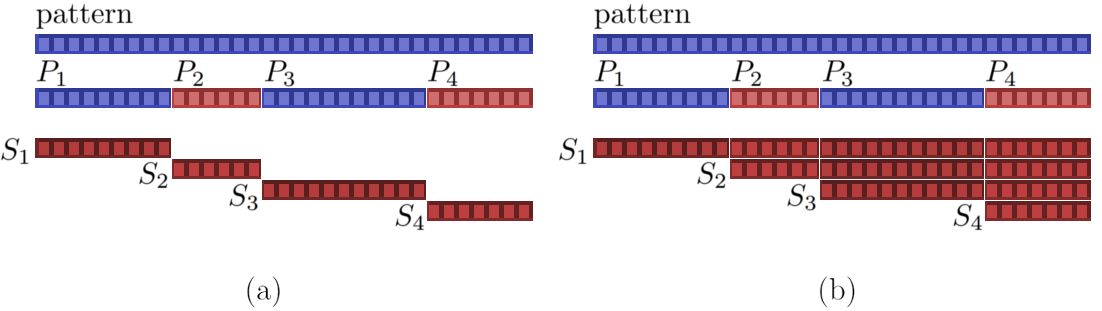
\includegraphics[width=1.0\textwidth]{images/substring_suffix.png}
\caption[Pattern string blocks vs. suffix block sequences for substring and suffix filter algorithms.]{Pattern string partitioned into blocks $[P_1, P_2, P_3, P_4]$, bringing rise to sequence of queries $[S_1, S_2, S_3, S_4]$. (a) Queries of the substring filter algorithm, one query per block of $P$. (b) Queries of the suffix filter algorithm, one query per suffix block sequence of $P$.}
\label{fig:substring_vs_suffix}
\end{figure}

As in the substring filter algorithm, the search process walks over query symbols one by one, keeping track of incrementally-longer \gls{match location} sets in the text throughout. Only now, the query string is comprised potentially of numerous blocks instead of just one. The search makes use of a parameter \bfit{pE} as it did in the indexed P2 algorithm, but this time it is initialized at $0$, effectively prohibiting any error-branching at first. Every time the search walk crosses over the end of a block, the search \textit{accumulates} a permitted error (i.e. incrementing \bfit{pE} by one); This alteration to the procedure effectively results in a limited version of the recursive branching seen in the indexed P2 algorithm from Section \ref{P2text_index}.

\begin{figure}[!htb]
\centering
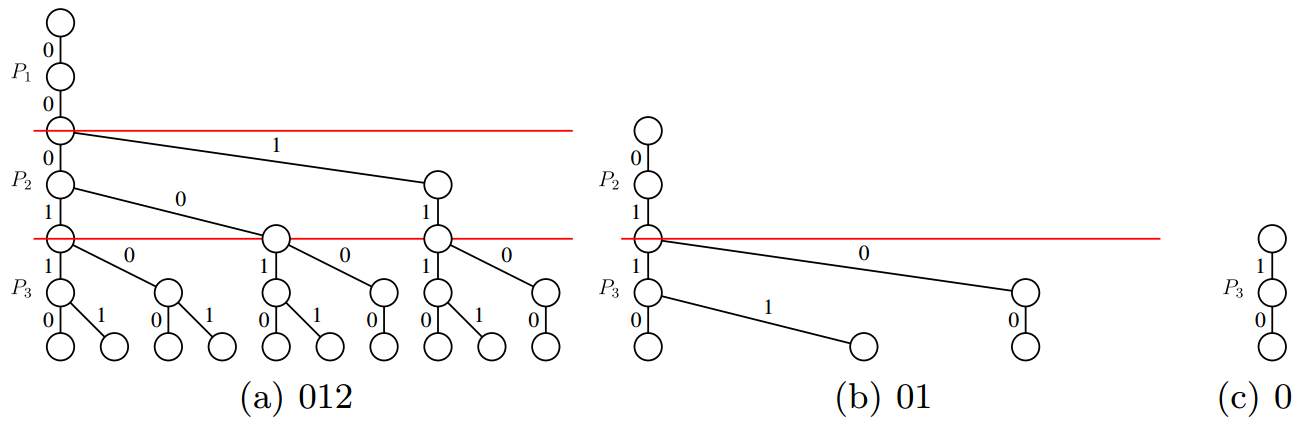
\includegraphics[width=0.92\textwidth]{images/trie.png}

\caption[Search trees from pattern `000110' using a binary alphabet, bringing rise to filters 012, 01 and 0 and three blocks, $P_1, P_2, P_3$]{Search trees\protect{}\footnotemark{} from pattern `000110' using a binary alphabet, bringing rise to filters 012, 01 and 0 and three blocks, $P_1, P_2, P_3$ (a) 3-block query for `100110' using filter 012. (b) 2-block query for `0110' using filter 01. (c) 1-block query for `10' using filter 0.}
\label{fig:filter_search}

\end{figure}
\FloatBarrier
\footnotetext{This Figure is taken from Kucherov \cite{kuch2014}}

% This algorithm relies on lemma \ref{lemma2} much like the substring filter algorithm relied on \ref{lemma1}; The lemma guarantees that for an arbitrary solution's match in the text $Y$, for at least one query, the branching behavior described above should be \gls{sufficiently lenient} such that it can match symbols all the way to the end of the pattern without eliminating the \gls{match location} for $Y$ from the set. As such, upon reaching the end of the the query string, the search generates a \gls{candidate}. Unlike the previous algorithm, many branches of the search tree may find their own such candidate sets. The return result of such a query is the union of all these sets.
 
The correctness of the suffix filter algorithm relies on the \textit{consequent} of lemma \ref{lemma2}. An arbitrary search query is \textit{not} guaranteed to find an arbitrary string $Y$ in the text; However, the lemma guarantees that \textit{at least one} search query for a suffix block sequence will have enough errors to spare throughout the search all the way to the end of the matching substring with $Y$ in the text, where it would generate a candidate to cover the \gls{solution} containing $Y$. As with the substring P2 algorithm, not all candidates necessarily correspond to solutions, as the search is `blind' to the symbols in blocks that prefix the first block of the query.
 
Observe that the suffix filters conduct a more \textit{thorough} search process, with blind sections for matches only on \textit{one} side, instead of on \textit{both} sides as was the case with substring filters. The suffix filter algorithm generally produces far fewer candidates, as it searches further to potentially thin out the match location sets than the substring filter algorithm does before generating candidates. Also observe that the \gls{search step} of the suffix filter algorithm takes longer, as it needs to spend more time searching more symbols \textit{with} recursive branching. In this sense, the suffix filter algorithm makes more extensive use of the text index than the substring filter algorithm.
\section{Solving P3: Approximate Prefix Match Using Suffix Filters}
\label{P3_suff}

Problem P3 is closely related to P2. However, instead of the \gls{pattern} being fixed, given as an argument directly, matches are found for any string $A$ that is any prefix of a given \gls{pattern} at least as long as the given \bfit{t}. At first glance, extending the \gls{suffix filter} algorithm for P2 seems simple; Indeed, the problem can be solved with several instances of P2 separately, one for each \textit{valid} prefix of the pattern playing the role of P2's input `pattern' (where `valid' is shorthand for `at least as long as \bfit{t}'). Although perfectly correct, this approach does not take advantage of the similarity between the prefixes; The beginnings of the \gls{text index} search \glspl{query} would repeat many of the same steps, duplicating work. Instead, \glspl{candidate} for each prefix can be located \textit{in tandem} without altering correctness; However, some care is required to preserve the premises of lemmas \ref{lemma1} and \ref{lemma2} on which the suffix filter algorithm is built.

% As described several times since section \ref{P2text_index}, throughout the search procedure of the text index, incrementally-longer prefixes of the query are \textit{matched}. Now, i

 
Instead of separate P2 problems, P3 can be approached as being more like a single instance of P2, where partially-completed query matches during the search may also represent desirable candidates (some nodes in the search tree mark the end of valid query prefixes). To implement this idea, the search procedure must be able to generate candidates when its progress corresponds with any \gls{derived string} of a valid query prefix.

During an index search, the degree to which the search node at an index position increments \bfit{pE} is a function of the sizes of the pattern's blocks; This requires the partition block sizes to be defined \textit{prior} to the search query's commencement. However, the correctness of the algorithm is reliant on every valid pattern prefix $A$ being divided into at least $K+1$ blocks, where $A$'s have various lengths and thus various values for $K$. This requires a single initialization for partition block sizes that sufficiently partitions all pattern prefixes finely enough at the same time. Although this is tricky conceptually, the partition can still be defined in terms of the pattern itself, as the \textit{error limit} for each of its prefixes is a predictable linear function of the prefix lengths (excepting for some rounding). This is the idea behind \vali{}'s \gls{partitioning scheme}; It seeks to identify a value \bfit{p}, the length of all pattern blocks (except for the last block, which can be smaller) such that no valid pattern prefix $A$ will have too few blocks and \bfit{p} is maximal. Kucherov's work describes their own partitioning scheme that satisfies this property, but distributes block lengths differently. These details are further explained in Section \ref{schemes}.


This algorithm for P3 is where the P2 `filter-free' text index algorithm from Section \ref{P2text_index} gets left in the dust. For long patterns, the text index search algorithm would need to permit very large initial values for \bfit{pE}, resulting in very deep and wide recursive search trees, branching far more than would be necessary to match the short prefixes of the patterns, but unable to avoid doing so in order to find the solutions for longer prefixes. The filter algorithms are able to leverage the \textit{incremental} introduction of \bfit{pE} to great effect for this reason, allowing for a much more appropriately \textit{gradual} introduction of errors, resulting in slimmer search trees.





\section{Solving the Approximate Suffix-Prefix Overlap Problem Using Suffix Filters}
\label{solving_ASPOP}

Where before the search space was defined by a given \gls{text} string, now the search space is defined by a given \textit{set} of strings $S$. Allowing for some bookkeeping steps before and afterwards, the \gls{text index} can be made to search these strings by being initialized with a text constructed from concatenated $S$ strings. Although it would cover all the solutions, unmodified, the above approach is too generous, as it would naively generate \glspl{candidate} anywhere within the constructed text (even overlapping two different $S$ strings). \Glspl{solution} would only exist as suffix positions for individual strings of $S$. Detecting these suffix positions is trivial if the text string is constructed with some distinct extra-alphabetic character delimiting the concatenated $S$ strings (conventionally `\$'). For example:
\begin{align*}
S &= \{\text{`TACC'}, \text{`GGG'}, \text{`ACCC'}\}\\
\text{text} &= \text{`TACCGGGACCC'}
\end{align*}

During the \gls{search step}, at the moment where the search is about to generate candidates from \glspl{match location}, an additional `\$' symbol is matched, effectively narrowing down the match location set to a subset that occur as $S$ suffixes; Only for all the match locations in this subset are candidates generated. The original match location set at this position remains unchanged and potentially continues the forward search, generating more candidates deeper into the search tree.
 
Aside from the alterations described in Section \ref{extensions} to support extensions, the above is the basis for the algorithms used to solve the \aspop{} onwards in the paper. As such, the \gls{suffix filter} solution to the \aspop{} as described in this section will henceforth be referred to as the `\aspop{} algorithm' for the `\aspop{} solver'.


\section{Suffix Filtering and Partitioning Schemes} \label{schemes}

\Glspl{suffix filter} allow a much faster search than the filter-free \gls{text index} search, and filter more thoroughly than \glspl{substring filter}, saving a lot of time in the \gls{verification step}. For these to result in an exact algorithm, the premises of the lemmas on which they are based need to be satisfied. This introduces requirements for the implementation of the \gls{filter criterion}, the \gls{partitioning scheme} of the \gls{pattern}, and determines when \glspl{candidate} must be generated throughout the \gls{query} searches to ensure to \glspl{solution} are missed. However, these requirements only \textit{bound} the possibility space for these algorithms, but do not specifically \textit{define} it; Design decisions arise that impact run time but not correctness. For instance, the suffix filter algorithm is only guaranteed to find all solutions when the patterns are divided into at least $K+1$ \glspl{block}. Partitioning into $K+2$ blocks satisfies the requirement, but profoundly changes the number of the text index \glspl{query}, the shape of each search tree, et cetera. Different choices for these design decisions result in different \textit{schemes}, many of which are explored thoroughly by \vali{} and Kucherov in an attempt to maximize speedup.



\subsection{Filtering Scheme Defined}
\label{schemes:def}

The \gls{search step} of any \gls{filter algorithm} is tasked with partitioning the search space into elements that satisfy the \gls{filter criterion} (\glspl{candidate}) and those that do not. How this set of candidates is \textit{found} is a matter that depends on the specific problem and its nature.
 
For \glspl{suffix filter}, elements in the search space, nodes in the search tree and string \glspl{derivation} of \gls{query} strings are all equivalent; Which branches are explored in a search determines the search elements encountered. For this reason, there is not complete freedom to use any branching behavior, but (as discussed in Section \ref{P3_suff}) the rules that ultimately determine branching need to be established such that they satisfy lemmas \ref{lemma1} and \ref{lemma2} to guarantee no solutions are overlooked. However, several conceivable such `branching behaviors' satisfy the lemmas. A \gls{filtering scheme} for the suffix filter algorithm defines a \gls{filter} for each query string's \gls{block sequence}, where a filter is simply a sequence of integers. During the search, each query block is associated with one filter value; Upon the search entering a new block, it uses the block's \textit{filter value} $fE$ to determine if and how much to increment \bfit{pE}, such that $sE+\bfit{pE}=fE$, where $sE$ is the error `spent' on the search node so far\footnote{As all \bfit{pE} could conceivably be spent at any time, by implication the numbers in a filter sequence are strictly \textit{nondecreasing} in the order they are encountered by the search.}. In this way, the contents of the filters define the branching behavior of query searches.

{the filter specifies a number for each block, interpreted as the maximum possible \bfit{pE} value entering that block during the search.
 
Consider the algorithm described in Section \ref{P3_suff} with some pattern $P$ divided into 3 blocks, and the search of the longest of $P$’s \glspl{suffix block sequence} (all 3 blocks) with filter $\{0, 1, 2\}$. The resulting search would initialize \bfit{pE} to 0, and increment \bfit{pE} by 1 at each subsequent block; This should look familiar, as it is the same scheme described in \ref{P3_suff}; This is \kark{}'s filtering scheme:

\begin{fscheme}[Karkainnen's Filters]
\textup{For a pattern with N blocks}
\label{karkfilters}
\begin{align*}
filters &= \{f_0, f_1\ldots{} , f_N\}\\
f_X &= [0, 1, 2,\ldots , X-1]
\end{align*}
\end{fscheme}


\subsection{Partitioning Scheme Defined}
The \gls{suffix filter} algorithms in this work have various requirements for the number of \glspl{block} in a \gls{string partition}; Indeed, even the one existing requirement for partition block sizes (discussed in Section \ref{P3_suff}) was only required to indirectly ensure a sufficient \textit{number} of blocks for all prefix strings. With this detail accounted for, the algorithms have no requirements on the \textit{size} of blocks. However, the shape of the search tree for a \gls{query} is a function of block sizes. For this reason, the choice of how a \gls{pattern} is partitioned greatly impacts cost of a suffix filter algorithm, and the rules that define these choices are called a \gls{partitioning scheme}.




\subsection{\kark{}'s Schemes}
\label{schemes:kark}

The \kark{} \glspl{suffix filter} had an efficient \gls{partitioning scheme}, suited for the problem they sought to solve (P2: `Approximate String Match' in Section \ref{solvingP2}), a simpler problem than the ASPOP. In their case, the length of the \gls{pattern} was known from the start. For this reason, the \gls{string partition} of pattern could be chosen to greedily minimize search time for that pattern and be the best choice overall.

For the \textit{substring filter} algorithm, the optimal string partition is obvious. As each \gls{filter} simply matches a single \gls{block}, the best speed is achieved with evenly-sized blocks. However, for \glspl{suffix filter} the choice is less clear, as evenly-distributed blocks do not result in work being evenly-distributed amongst filters.

\kark{} observed that \glspl{query} that started in a short block had fewer opportunities to narrow down their \glspl{match location} before starting to generate \glspl{candidate} (once the first block was completely matched), which manifested in such queries generating storms of spurious candidates. These factors suggested that a good scheme required a balance to be struck between \textit{preventing short blocks} (a pressure to evenly-distribute block lengths) and to \textit{balance the work of each filter} (a force to make the right-most blocks longer than the left-most blocks). \kark{} opted to make the \textit{last} block longer than the rest, with the other $K$ blocks dividing up the remaining length as evenly as possible. \kark{} observed that this alteration to the partitioning scheme had a positive effect on the runtime of the algorithm, but they could not find a trivial way of optimizing the choice of length for the last block, resigning it to be determined experimentally on a case-by-case basis.


\subsection{\vali{}'s First Schemes}
\label{schemes:vali1}

The first \vali{} paper attempted to most-directly adapt \kark{}'s \gls{suffix filter} algorithm for the \aspop{}, using filtering scheme \ref{karkfilters} (\kark{}'s filters).

\vali{} recognized the potential of searching all prefixes of strings in parallel and were forced to adapt the \gls{partitioning scheme} in accordance to the new correctness constraints imposed by this choice (as described in Section \ref{P3_suff}). To ensure every \textit{valid} prefix was divided up into at least $K+1$ blocks, \vali{}'s approach provides a formula to determine the largest choice for uniform block length that would not overlook any prefixes for the given \gls{pattern} size. Keeping block lengths largely uniform was carried over from the \kark{} implementation. This was a logical choice to always increment \bfit{pE} at the last possible moment in the search in order to minimize the width of the search tree. As identified by \kark{} in their own work, this design had an optimally-short \gls{search step}, but created very many spurious \glspl{candidate} that would increase time taken in the \glspl{verification step}. The use of a predefined block size presented a problem when used for the \aspop{}; Very many indices in the pattern (in fact all indices larger than \bfit{t}) correspond with the end of some \textit{valid} prefix; For simultaneous searches for all prefix matches (as described in \ref{P3_suff}), a prefix might end part-way through some pattern block, cutting that block short; This is shown in Figure \ref{fig:short_block}. When seen in isolation, such a prefix would have a short final block (in the worst case, the final block would be only 1 symbol long!) and the final filter would generate many spurious candidates. This situation arises in every partitioning scheme with any block division occurring after \bfit{t}.

\begin{figure}[!htb]
\centering
\makebox[\linewidth][c]{%
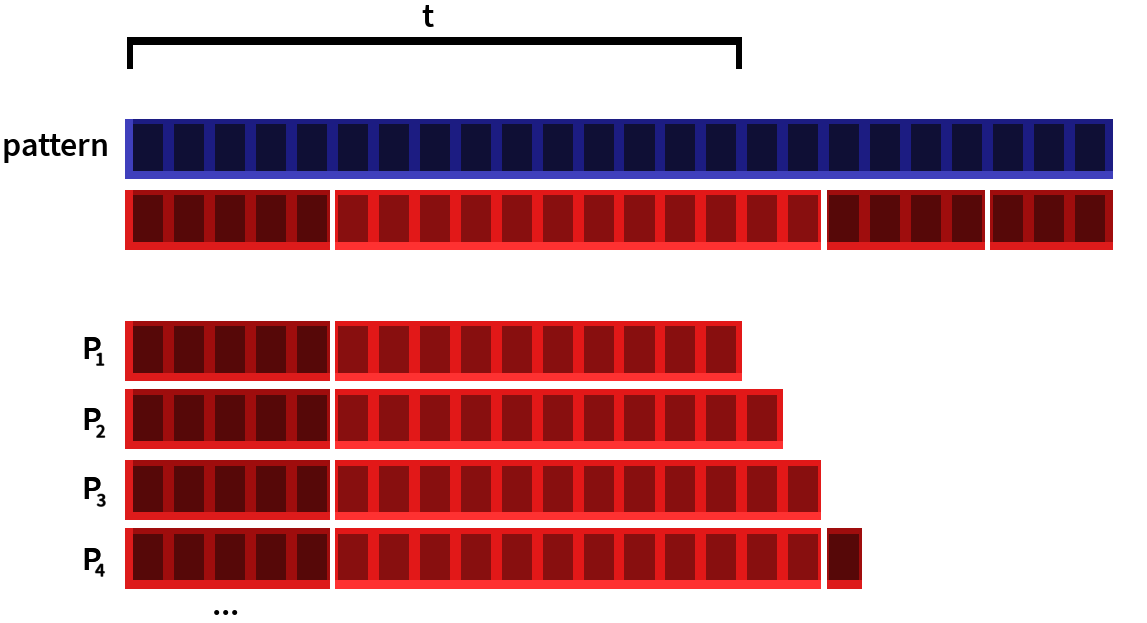
\includegraphics[width=0.7\textwidth]{images/short_block.png}
}
\caption[Short final block in some prefix of a pattern demonstrated]{Prefixes $P_1...P_4$ of some pattern string, where the length of $P_4$ induces a short final block from the pattern's block sequence.}
\label{fig:short_block}
\end{figure}
 
To remedy this problem, \vali{} had a number of ideas which involved passing over the same prefix a number of times, each time offsetting the partitioning divisions on the pattern, and selectively disabling candidate generation whenever these short blocks were predicted to arise. Without dwelling too much on the specifics, this approach was able to cumulatively cover all \glspl{solution} and avoid having to output candidates in cases with extremely short queries. However, it required several passes over the same pattern.





\subsection{\vali{}'s Second Schemes}

\label{schemes:vali2}
Following up their previous paper, \vali{} proposed a new \gls{filtering scheme} to sidestep the problem of short \glspl{block} that plagued their previous algorithm.
 
\begin{fscheme}[Valimaki's Filters]
\textup{For a pattern with N blocks}
\label{valifilters}
\begin{align*}
filters &= \{f_1, f_2\ldots{}, f_{(N-1)}\}\\
f_1 &= [1, 2,\ldots , N]\\
where\phantom{ }X \neq 1 : f_X &= [0, 1, 2,\ldots, X-1]
\end{align*}
\end{fscheme}

\noindent
The new filtering scheme had a new desirable property; To cover all \glspl{solution} for any \gls{pattern} of $K+1$ blocks, the very shortest \gls{filter} (composed of a single block) could be entirely omitted. For the algorithm, this meant that a solution for any prefix of the pattern would be covered even if all searches did not generate \glspl{candidate} until the end of the complete first block. The new algorithm was able to output candidates in just one \gls{text index} \gls{query} per filter. To cover cases that would ordinarily only be found by the missing \gls{query}, the first (largest) \gls{filter} that all prefixes would have in common has its \bfit{pE} 1 larger in all positions than in filtering scheme \ref{karkfilters}; This can be achieved in the search by initializing $\textit{pE} = 1$ instead of 0, giving the branching a head start. As a consequence of the wider search tree, more time is spent in the \gls{search step}. However, the increase in search time is vastly outweighed by the \textit{decrease} in time spent in the \gls{verification step} when using filtering scheme \ref{karkfilters}.






\subsection{Kucherov's Schemes}
\label{schemes:kuch}

In the fashion of \vali{}'s second paper, Kucherov attempted to make an improvement to the earlier algorithm of \vali{}'s first paper by fixing the short first \gls{block} problem. Kucherov offered a new \gls{filtering scheme} that achieved this in a new way.

\begin{fscheme}[Kucherov's Filters]
\textup{For a pattern with N blocks, given a positive integer $S$}
\label{kuchfilters}
\begin{align*}
filters &= \{f_0, f_1\ldots{}, f_{(N+S-1)}\}\\
f_X &= [0, 1, 2,\ldots , X-S]
\end{align*}
\end{fscheme}

Instead of each prefix having $K+1$ partition blocks (for error limit $K$), Kucherov's solution relies on $K+S$ blocks for each prefix, with $S\geq2$. This could be interpreted as guaranteeing $S$ error-free blocks up from just one. This change increases the breadth of search trees, but avoids many \textit{spurious} candidates from being generated, thereby saving time in the \gls{verification step}; The key observation is that the unavoidable \textit{short last block} can now no longer be the \textit{only} block matched for any candidate; Hence, no candidate will be generated with less than one \textit{complete} block's worth of symbols matched.

The correctness of this algorithm can be seen from lemma \ref{lemma0}, a more generalized version of lemma \ref{lemma1}.

\begin{lemma}
\label{lemma0}
If a string containing no more than $K$ symbols $\phi{}$ is partitioned into $K+S$ blocks for $S \geq 0$, at least $S$ blocks must have $0$ $\phi{}$'s.
\end{lemma}

In Kucherov’s canonical example, $S=2$ (where $S=1$ in \vali{}’s first algorithm), but any positive value of $K$ remains correct. With more finely-partitioned prefix patterns, the \gls{filtering scheme} could safely assume that each \gls{solution} would contain more \gls{error}-free blocks, and match more blocks before generating \glspl{candidate}. So far, the assumption of the 0-error blocks occurring as the \textit{first} block in each query only holds because queries are generated to exhaustively guarantee the correctness of the algorithm \textit{using all} queries (essentially branching into a \textit{case distinction} for which each case covers one position for the 0-error block). Creating queries relying on the \textit{specific} position any \textit{subsequent} 0-error blocks in the \gls{block sequence} (for example, the 2nd of two for $S=2$) would require \textit{another} layer of case-distinction, resulting in a number of filters and queries quadratic in the number of blocks, rather than linear. To avoid this, the position of subsequent blocks is not nailed down at all, and \bfit{pE} continues to be incrimented until the last possible moment; In effect, this simply requires that 0-error blocks number 2 to $S$ occur \textit{somewhere} in the block sequence after the first 0-error block. This reasoning is based on lemma \ref{lemma2}.

In addition to guaranteeing more complete blocks matched per candidate, increasing $S$ results in more balanced (albeit increased) work across filters. In a sense, small values of $S$ cause the algorithm to approach the \kark{} algorithm, while large values of $S$ cause it to degenerate towards the filter-free \gls{text index} algorithm from Section \ref{P2text_index}; (The advantage of using blocks at all falls away as blocks get shorter.)
 
In the previous filtering schemes with uniformly-increasing \bfit{pE}, \glspl{filter} of all lengths were prefixes of one another. This is not the case for these Kucherov filters. For searches intended to traverse all prefix lengths (and thus, apply all lengths of \gls{suffix filter}) in tandem, this requires the search path to \textit{fork} at each new block, with some branches accruing an extra \bfit{pE}, and others matching $S-1$ blocks, generating candidates and terminating. Figure \ref{fig:pE_fork} demonstrates this branching search path for $S = 2$. 


\begin{figure}[!htb]
\centering
\makebox[\linewidth][c]{%
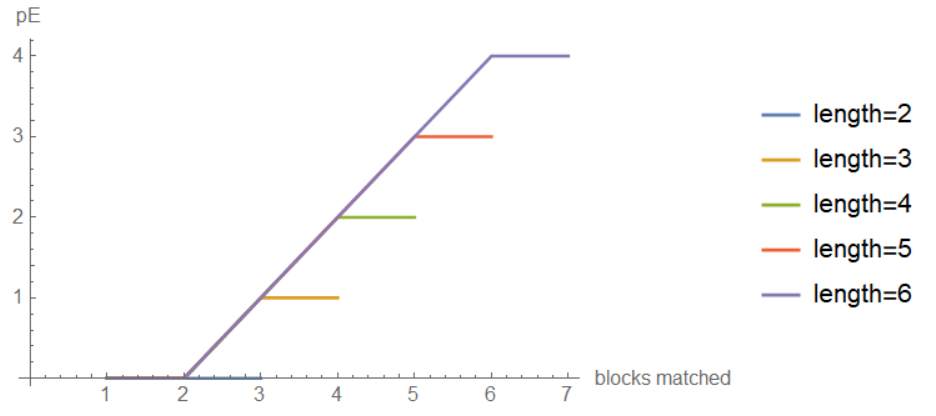
\includegraphics[width=0.8\textwidth]{images/pE.png}
}
\caption[Permitted error variable at various depths in the search tree for per filter length.]{Variable \bfit{pE} `permitted error' at various depths in the search tree (measured per block) for different filter lengths.}
\label{fig:pE_fork}
\end{figure}

Instead of forking the search path, the \gls{candidate condition} can be strengthened to suppress candidate generation for search branches with $\bfit{pE} < S-1$; This achieves the same result of forking the branches, but requires a constant-time check instead of actually forking branches.


\section{Algorithm Extensions}
\label{extensions}

The work in the \vali{} and Kucherov papers focuses primarily on the most fundamental aspects of solving the \aspop{}. Extensions exist that facilitate discovery of additional \glspl{solution}, namely \glspl{inclusion}, those brought about by consideration of \glspl{reversal}, as well as support for \gls{edit distance} as an \gls{error distance} measure. As none of these extensions change the fundamentals of the algorithms, \vali{} and Kucherov don't delve too deeply into how they should be implemented. However, the use of these extensions factors greatly into runtime, as well as requiring a significant amount of original work to implement them into the \aspop{} solver effectively.



\subsection{Edit Distance}
\label{editdistance}

\Gls{insertion} or \gls{deletion} \glspl{error} are often given the general name `\glspl{indel}'. For realistic applications in genome assembly, it is sometimes advantageous to consider \gls{edit distance}  instead of \gls{Hamming distance}), as it is defined for strings of different lengths and is more representative of the ways single-symbol errors can by physically introduced when reading genomic information. The support for these indel operations necessitates changes in both steps of the \gls{suffix filter} algorithm:

\begin{enumerate}
\item Changes to the \gls{search step}

The search procedure needs to allow branches that represent indel errors in the \gls{derivation} of match strings from the \gls{query} string. These added error operations manifest as a new set of recursive calls at each node in the search tree.

\item Changes to the \gls{verification step}

The computation to measure the error intrinsic to a \gls{candidate}’s overlap needs to be in terms of edit distance.
\end{enumerate}

Indels differentiate the lengths of the overlapping components $A$ and $B$ between the \gls{pattern} string and its \textit{match string} in the \gls{text} respectively; \Glspl{insertion} increase the length of $B$ without changing the length of $A$; \Glspl{deletion} increase the length $A$ without changing the length of $B$. These added operations necessitate that both two lengths be decoupled and stored \textit{separately} in each symbol-step of the \gls{text index}'s recursive \gls{query} search. Concepts such as \gls{string partition} size and permitted errors are defined in terms overlap length; At first glance this seems to present a circular definition, with each indel error influencing how many indel errors are permitted (by changing overlap length). Fortunately, this problem can be resolved due to the \gls{error rate} limit parameter (\bfit{e}) being strictly lower than 1, where a lengthening \gls{derived string} will always run out of errors faster than it accumulates length from errors (in the most extreme case, all errors are insertions, increasing length); This assures a hard cap for the length of derived strings.
 
In addition to complicating the algorithm conceptually and requiring further checks, the permission of indels greatly increases the branching factor of the query search, as simply more derivation branches are possible at each node in the search tree with the added operations. Thankfully, some branching \textit{rules} can be incorporated to curtail this branching factor without affecting the correctness of the algorithm. For instance, a rule could prohibit a deletion at index $N+1$ if there was an insertion at index $N$ in the same search path. Any \glspl{candidate} generated by nodes within the subtree with its root at index $N+1$ would also have been found by the subtree resulting from a \gls{substitution} at index $N$; No candidates will be overlooked by enforcing this branching rule. Many other such rules can be introduced to avoid redundant work in each search in this manner.


\subsection{Reversals}
\label{reversals}

The consideration of \glspl{reversal} comes from an application perspective. For genome assembly, \gls{read} strings in the input set $S$ are collected by reading nucleotides that are encountered when passing over a strand of \textsc{dna} or \textsc{rna} (some genomic material). In some instances, this strand is tightly bound to another companion strand, with connections at each nucleotide. Such nucleotide \textit{base pairs} always couple symmetrically and predictably, with `A' pairing with `T' and `C' pairing with `G'. Although this other strand is not read, its nucleotide sequence can be \textit{deduced} by leveraging the knowledge of its companion (which \textit{is} read). In this event, the algorithm can internally consider two strings per input string in $S$ (one given string, and one companion string) to find new overlaps involving these reversals.
 
The use of reversals has a similar impact on runtime as the use of an $S$ set twice the size. Additionally, some care must be taken as with two \textit{versions} of each read in the \gls{text}, the same solution could be found twice. Some minor bookkeeping is needed to avoid or resolve this duplication; The approach used in our implemented \aspop{} solver is detailed in Section \ref{impl:dedup}.






\subsection{Inclusions}
\label{inclusions}

\Glspl{inclusion} are a class of overlap \gls{solution} between two strings different to the suffix-prefix overlaps considered thus far. Some string $A$ is \textit{included} within some string $B$ if $A$ matches a substring of $B$. As before, this concept can be extended with the use of \glspl{error} to define a \gls{K-approximate} inclusion.
 
Knowing that two \glspl{read} came from the same genomic sequence facilitates some confidence in the correctness of the read symbols, provide redundant symbols for error correction, and helps the estimation of read `quality' (probability of misread symbols). In addition to suffix-prefix overlaps, inclusions can find such overlapping reads.
 
Extending the \aspop{} \gls{suffix filter} algorithm to also find inclusion \glspl{solution} can be done in a number of ways. One such way involves a minor change to the \gls{text index}'s search procedure. \Glspl{candidate} are now generated at the very last index of the search \gls{query} whether or not they are followed by a `\$' symbol in the \gls{text}. These special candidates would represent an occurrence of a \gls{derivation} of the \textit{entire} query string somewhere in the text (not only as the suffix to some $S$ string). The \glspl{match location} for generated candidates likely do not align with `\$' positions in the text; Thus determining to which $S$ string the match location belongs presents a minor computational challenge. Many approaches are possible, but we suggest a binary search over the known `\$' indices in the text, matching the largest `\$' index that is smaller or equal to the found index; Knowledge of which `\$' string to associate with the match location provides enough information to determine which $S$ string is associated with the found overlap, and consequently, affords the generation of a candidate;
 
Under most circumstances, allowing for inclusions greatly increases the number of candidates generated and thus increases the time taken to complete the \gls{verification step}. To see this in action, refer to Section \ref{extension_runtimes}.
\chapter{Custom Implementation}

\section{Program Structure}
\label{structure}

Our goal was to develop a fast \aspop{} solver that would adhere as closely as possible to the literature described in Section \ref{background}, along with the extensions described in Section \ref{extensions}. For the purpose, our system was implemented in the Rust\footnote{Available at \url{https://www.rust-lang.org/en-US/}} programming language, chosen mostly for it's thread-safety and the systems-language speed it provides \cite{rustlang}.

The implementation was structured around an isolated \textit{mode} module that would act as an interface for altering the behavior of the \glspl{filtering scheme} and \glspl{partitioning scheme} for testing; The mode component would define functions to determine:
\begin{enumerate}
\item Pattern partition sizes
\item Filtering scheme
\item Candidate generation condition
\end{enumerate}

Depending on the definition of these functions, the program would implement the schemes of \vali{} and Kucherov, along with any experimental schemes of our own. The idea was to make the program’s behavior as consistent as possible between different modes such that they could be compared and benchmarked experimentally. Additionally, this modular approach allowed for faster iteration on testing of new schemes.
 
The pseudo code in Figure \ref{fig:pseudocode} gives a high-level overview of the program’s processes, which abstracts over the two steps of the algorithm for a single pattern string from the $S$ set as a task. The effects of the mode component are limited to the \gls{search step} of each \gls{task}.

\begin{figure}[!htb]
\centering
\myPython{data/pseudocode.py}
\caption[Python pseudo code for the implementation of the \aspop{} solver.]{Python pseudo code for the implementation of the \aspop{} solver, with details such as multi-threading omitted for brevity.}
\label{fig:pseudocode}
\end{figure}












\section{Additions to the Literature}

\subsection{Resolving Opposing Search Directions} \label{own_impl_search_dir}

The \aspop{} implementation makes use of a conventional \textit{FM-Index} \gls{text index} (See \ref{fmindex}). Due to the nature of the underlying \textsc{bwt} (See \ref{bwt} for more details), the text index is ultimately only capable of matching symbols when searched from \textit{right} to \textit{left}. The existing literature set a precedent of describing the \gls{suffix filter} algorithm \gls{search step} in a forwards direction (from the front to the back of the \gls{pattern}), which results in suffix filters instead of prefix filters.
 
The difference in terminology here (left and right vs. front and back) is deliberate.
 
In this \aspop{} implementation, $S$ strings are indeed searched from front to back, but the front of the strings lie \textit{right} of the back of the strings, in terms of index positions and so forth. \vali{} refer to this as a `simulated forwards search' \cite{vali2010}. This unintuitively-reversed representation satisfies the requirements of the FM-Index as well as the precedent of the literature for suffix filters at the same time. To minimize duplication of data, this `inverted' internal representation is sustained for the entirety of the execution (allowing for trivial mappings from string \textsc{id}s to indices in the text) except for the outward-facing interfaces of the solver, namely the algorithm \textit{mode} module and the eventual program output. The end user doesn’t have to be aware of this inversion to make full use of the system, but it is relevant for understanding the relationship between the inner workings FM-Index and the suffix filter algorithm.
 
Note that there exist other viable methods of achieving the same results without this inversion \cite{lam}.




\subsection{Deduplicating Candidates}
\label{impl:dedup}

When reversals are enabled (See Section \ref{reversals}), the \gls{text} is constructed from two strings per read in the input $S$ set, one normal string $X$ as would be expected, and one companion reversed string $X'$. As a result, when performing the \gls{search step}, some \gls{solution} might be located twice; Once from $X \rightarrow Y$ and once from $Y' \rightarrow X'$ (or once from $X \rightarrow Y'$ and once from $Y \rightarrow X'$). This necessitates some effort to deduplicate the \gls{candidate} set. Ideally, this deduplication should be done before the \gls{verification step}, as performing redundant verification work is wasteful. Detecting and discarding these duplicate candidates can be done if strings comprising the \gls{text} are given ordered \textit{\textsc{id}s}; Leveraging the fact that these duplicate candidates are always found with inverted orderings of the respective \gls{pattern} and \textit{match string}, one of the two \gls{task} can suppress the generation of the candidate, safe in the knowledge that its companion task will not; The companion task will encounter an inverted \textsc{id} ordering. Either choice of suppressed ordering would work, as long as a convention is respected consistently across tasks.
 
Other more intuitive and robust means of deduplicating overlap solutions can be done if threads are allowed to communicate or otherwise pool their solutions or candidates. As this approach introduces overhead, it was avoided in our implementation.





\subsection{Defining Overlap Length for Edit Distance}

When using \gls{edit distance} as an \gls{error distance} measure, the notion of an \textit{overlap length} becomes less trivial to define; An overlap could be constituted of two substrings of different lengths. The precise definition of an overlap length is necessary for the \gls{verification step}, as the specific permitted error limit `$K$' is a function of this length (from the given error rate limit argument \bfit{e}). For realistic applications, as \glspl{indel} are rare enough not to differentiate lengths in an overlap, and the choice of \bfit{e} is likely to be a ballpark estimate anyway, this may seem like a pedantic point to dwell on. However, from a correctness perspective, even minimal differences in the definition of `overlap length' would change the \gls{solution} set.

For our implementation, the more generous approach is taken, validating \glspl{candidate} using the \textit{maximum} of the two overlap lengths to determine the discrete error limit. This has the advantage of preserving the symmetric nature of edit distance.



\subsection{The Unknown Overlap Length Problem}
\label{unknown_b}

With consideration of \gls{edit distance} and the \gls{indel} \glspl{error} that come with it, some values needed for the \gls{verification step} are not so easily given as they are when indels are not permitted. This requires some extra work, the manner of which creates a design decision and runtime dependent on how the problem is solved.

Consider some candidate $C$ generated from some element in the \gls{match location} set of a node in the \gls{query} search tree. $C$ represents a potential overlap \gls{solution} between some \gls{pattern} string $X$ and some other string $Y$. In the usual \aspop{} fashion, some \textit{prefix} $A$ of $X$ is therefore a \gls{K-approximate} match to some \textit{suffix} $B$ of $Y$ (for some sufficiently-low $K$ value). The query search that generated $C$ did not necessarily begin searching from the very first symbol of the pattern. In fact, all but the first query (and associated \gls{filter}) for any pattern are \textit{blind} to the symbols in some non-empty prefix of that pattern. For $C$ to have been generated, this \textit{blind} section must have been some strictly-shorter prefix sequence of $A$, or else the search path will have had an empty (or negative?) length; As such, let $A$ be partitioned into a prefix $A_p$ and suffix $A_s$, where only $A_s$ symbols were matched during the search. Similarly, let $B$ be partitioned into $B_p$ and $B_s$, with all query \gls{derivation} symbols falling into $B_s$. Figure \ref{fig:blind} should help to visualize the relationship between these variables.

\begin{figure}[!htb]
\centering
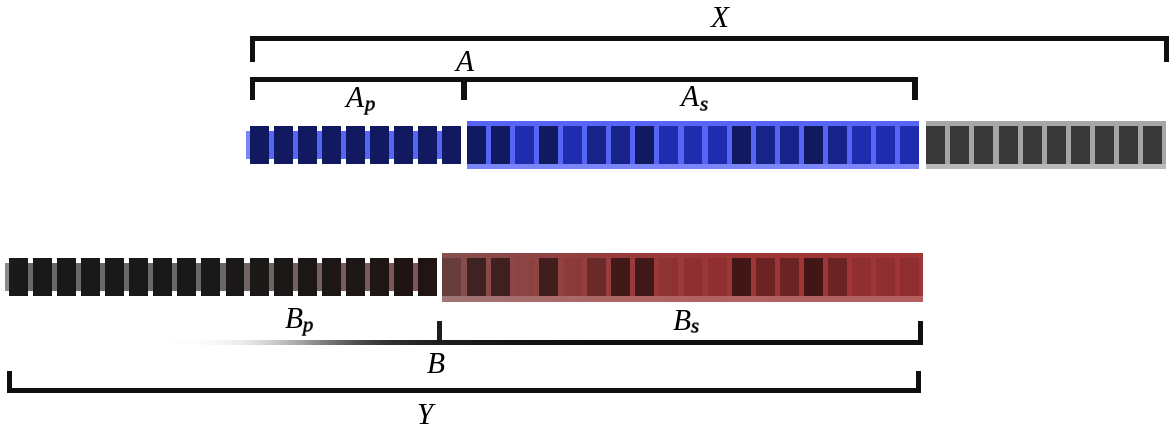
\includegraphics[width=.8\textwidth]{images/blind.png}
\caption[Overlaps between two strings $X$ and $Y$, illustrating the portion of the overlap with an unknown length.]{Some overlap between strings $X$ and $Y$, with overlapping sections $A$ and $B$, each of which is divided into prefixes $A_p$ and $B_p$ respectively and suffixes $A_s$ and $B_s$ respectively. The length of $B_p$ is unknown if the distance between strings is defined in terms of edit distance.}
\label{fig:blind}
\end{figure}

Observe that the known symbol-offset into $X$ of the query string implicitly defines the boundary between $A_p$ and $A_s$; Thus, these substrings have known lengths $|A_p|$ and $|A_s|$. Length $|B_s|$ is also known, as the search process could easily record and manipulate local variables on the stack to keep track of the string \glspl{derivation} associated with each node in the search tree.


In the event of \gls{Hamming distance} being used as the \gls{error distance}, by definition $|A|=|B|$. Therefore, both overlaps comprising $C$ are known, and can be used for the \gls{verification step}. However, using \gls{edit distance} as the distance measure, the same property does not hold. Although $|B_s|$ is indeed known, the same cannot be said for $|B_p|$. Thus, it becomes unclear where to draw the boundary between the suffix $B$ of $Y$ and the rest of $Y$ not involved in the overlap. Of course, possible values for $|B_p|$ are constrained by the length of $Y$; Clearly the overlap length cannot exceed the length of the strings involved. Even better, the $|B_p|$ is obviously related to $|A_p|$, and as the number of indels between $X$ and $Y$ is restricted, the difference in length between these two substrings is also restricted. Still, a candidate with non-specific overlap length(s) cannot be verified.

It would appear then that the only way to cover all solutions is to consider all possible values of $|B|$ within the bounds, and generating a separate candidate for each possibility; Indeed, this approach is quite practical if the \gls{error rate} limit is expected to be low (resulting in a tight bound). Consider a string $X$ with an overlap length of 50 characters, using an error rate limit of 2\%. A naive estimate bounds the length of $Y$'s overlap to the small range of [49, 51]; Any other lengths would necessitate more \glspl{indel} than would be permitted. Knowledge of how many errors are known to exist between $A_s$ and $B_s$ can serve to tighten this bound even further. Continuing our example, just one error between $A_s$ and $B_s$ would imply with certainty that $B_p=50$ for the overlap to have a hope of verifying.

In our \aspop{} solver implementation, exactly this range method is used, potentially generating a handful candidates per \gls{match location} when edit distance is used as the distance measure.
 
Another more robust solution would necessitate a modified \gls{verification step} and candidate representation, where each candidate stores the \textit{range} of lengths for $B$. A well-known dynamic programming algorithm for edit distance could be altered to return distance values for all overlap lengths in this range in tandem. This, however, would necessitate further complicating the implementation and cluttering the system with complex deduplication methods to resolve candidates that contain overlapping overlap ranges.




\subsection{Modified Edit Distance}
Many applications of an \aspop{} solver are interested in the lengths of the prefix and suffix of strings in overlaps; For instance, longer overlap \glspl{solution} are less likely to be \textit{false}, only being facilitated by some `lucky' read \glspl{error}.
 
The standard \gls{edit distance} measure allows for \glspl{insertion} or \glspl{deletion} at either end of an overlap. This runs counter to our understanding of a `real' overlap. With available indel errors to make, the \gls{query} search would indiscriminately retain solutions that are only possible by `padding' the ends of the overlap with inserted symbols to extend the overlap length as much as \bfit{pE} will allow. This might exaggerate the degree to which two strings overlap. To mitigate this, our implementation uses a \textit{modified} edit distance function, wherein the very end symbols of overlaps are prohibited from being the result of insertions or deletions. A byproduct of this decision renders the edit distance between very short strings (such as strings `GGG' and `GG') undefined, with no way to go from one to the other without violating the new rule. In practice, good solutions are required to be substantially longer by the \bfit{t} parameter anyway, so this requirement doesn't cause any solutions to be overlooked.
 
Accepting this modified edit distance allows for increased strictness for the \gls{candidate condition}, reducing the number of generated candidates via redundant search paths. Whenever a search step most recently performed an insertion or deletion, it suppresses candidate generation for one step; Any candidates for solutions thereby overlooked in such a suppressed search node must be reachable with another, and will yield a candidate in that node instead of doing so in both. In this way, the modified edit distance defines the solution set to miss just a few elements, but cuts down a significant number of redundant candidates.







\section{Complexity}
\label{complexity}

\vali{} offer some time and space complexity bounds for a problem of this nature in general and for the \gls{text index} search discussed in Section \ref{P2text_index} \cite{vali2012}. In this section, we attempt to bound the time complexity specifically when using a \gls{suffix filter} algorithm. We also discuss the behavior one can expect from the implementation in terms of space.

\subsection{Time Complexity}
\label{time_complexity}



Often \glspl{filter algorithm} have abysmal worst-case time complexities, but tend to do significantly better in the average case \cite{kuch2014}; This is a consequence of the foundations of their \glspl{filter criterion} relying on assumptions about the problem instance that experience tells us are extremely likely to hold. In our case, actual runtime is sensitive to a host of variables including inherent properties of the input data set itself (as can be seen from the experiments in Section \ref{phase2}).

Key to the runtime of \textit{both} steps of the \gls{suffix filter} algorithm is the shape of the \gls{query} search tree in the \gls{search step}, as this determines the time complexity of this step, but also the number of candidates; Consequentially, this also determines the time spent in the \gls{verification step}. For this reason, we attempt to bound the \textit{number} of nodes in the entire search tree for an arbitrary \gls{query} search, and reason forward from there. This bound is given as:
$$\mathcal{O}(b^2 \cdot{} a^b \cdot{} l^b \cdot{} b!)$$

where\\


% \\[3mm]
\vspace{-2mm}
\hspace{0.6cm}
\begin{tabular}{lcl}
$l $ &:& length of the longest block in the \gls{pattern}\\
$b $ &:& number of pattern blocks i.e. $b=K+1$\\
$a $ &:& \parbox[t]{8.3cm}{number of symbols available for a \gls{mismatch}. i.e. $a=|\sigma{}|-1$ for symbol alphabet $\sigma{}$}
 \end{tabular}
\\[3mm]

To arrive at this expression, we have made the following assumptions:

\begin{itemize}
\item No branch in the search tree is ever \textit{pruned}. Indeed, this is only reasonable in the worst case and should be interpreted as such. Realistically, branches being regularly pruned is the assumption that the entire \gls{filter algorithm} relies on to offer an advantage. Unfortunately, for arbitrary \glspl{text}, we can make no such assumption.
\item The algorithm uses the simplest of \glspl{filtering scheme} (that of \kark{}) with only one redundant block per pattern prefix so lemma \ref{lemma1} is satisfied minimally.
\item Blocks are of equal lengths. Indeed this is very unrealistic, but this is the effect of using this bound. In reality, some blocks are shorter than the defined $b$. This fact makes our upper bound more \textit{conservative} than is strictly necessary. However, assuming the basic \vali{} \gls{partitioning scheme} this assumption holds for all blocks but one; All blocks have some \bfit{p} length, except the last which has some length $x$ in $1\leq{}x\leq{}\bfit{p}$.
\end{itemize}

Understanding this bound and how it was composed is best-done by breaking it down and enlisting the help of two smaller subproblems:

\begin{enumerate}
\item \textbf{Number of nodes in a 1-block long tree with $\bfit{pE}=m$}

The search performed by the \gls{text index} is structured as a branching tree of string \glspl{derivation}, with nodes for each derived prefix of the query (and thus, substring of the pattern). Each node (and each symbol) involved falls into a particular pattern \gls{block}. The total number of nodes in the search tree is what we are after, but this term can be further decomposed into the number of nodes \textit{within} a certain block.

Consider the first block with $\bfit{pE}=0$. The search path can do nothing but linearly walk the block to the end, requiring $l$ such steps. Thus, this block contains $l$ nodes.

For a tree in a block given $\bfit{pE}=1$, the search steps through $l$ symbols in the block's string, at each step producing $|\sigma{}|=a+1$ branches in total (with $a$ branches for an error-introduction steps + 1 step for matching the query symbol). The resulting child-branches of error steps have $\bfit{pE}=0$ and thus can do no more than to walk to the end of the block much as the first $\bfit{pE}=0$ block did. The number of nodes in this subtree is $l+a\cdot{}((l-1)+(l-2)+...+1)$, as each linear subtree from each error has a shorter distance to go the later it forks off from the 0-error path.

Lastly consider the case of a search beginning in a block with $\bfit{pE}=2$.  Along with the usual single 0-error linear walk to the end, each symbol position can introduce an error and bring rise to the $\bfit{pE}=1$ block problem described above, but with a `shorter block', so to speak. This manifests itself as a 2-dimensional summation series:
$$l + a\cdot{} (a((l-1)+(l-2)+...+1) + a((l-2)+(l-3)+...+1) +...+ 1 )$$
With each increase in \bfit{pE}, the dimension of this series is incremented; Conceptually, each increase instantiates $a\cdot{}l$ instances of the subproblem with one less \bfit{pE} and a `new block length' of however many symbols lie between the current index and the end of the block. Even the base case of $\bfit{pE}=0$ can be written as $l + a\cdot{}(0+0+...+0)$. In this fashion, the number of nodes in such a 1-block-long tree for arbitrary $\bfit{pE}=m$ is in the order of: $$\mathcal{O}(a^m \cdot{} l^m)$$




\item \textbf{Number of leaves in a tree ending after the $n$th block having spent $m$ errors so far}

We are also interested in how many \textit{leaf nodes} exist at the end-boundary of a given block, and how many errors those nodes have spent so far; These nodes will be roots of subtrees in the subsequent block.

Consider the base case of a tree for a block with $\bfit{pE}=0$. As before, all that the search can do is walk forward, with no branching whatsoever, so this tree ends up reaching the end of its block with just one 0-error leaf.

Next, consider a tree comprised of two blocks. As before, the unique path without any error-branching is always an option, and will produce a single 0-error leaf at the end of the 1st block, as well as the 2nd block. Once beyond the first block, the search can recursively consider positions to spend its stored \bfit{pE}, each time introducing an error in $a$ unique ways. This is possible in every index of the second block; Each resulting child branch will have no more \bfit{pE} to spend, forcing it to simply match the remaining query symbols linearly. In total, this tree will have $l \cdot{} a$ such 1-error branches.

For one last step, consider adding a third block. This tree has the single ever-present 0-error node at the end of the 2nd block. Any 1-error paths could only have forked from the 0-error path in the second or third blocks, resulting in $2 \cdot{} l \cdot{} a$ 1-error leaves. As errors are introduced sequentially, it can be reasoned that any 2-error path at some point forked off a 1-error path. This fork could have occurred at any index using any of $a$ symbols, but entirely \textit{after} the second block, as prior to this there is insufficient \bfit{pE} to introduce the second error. As such, there will be $2 \cdot{} l \cdot{} a$ such 2-error leaves.

The same reasoning allows us to enumerate the kinds of leaves for some $m$th block. Assuming that the maximal number of errors is smaller than $l$ (a reasonable assumption), the branching can occur at any index in blocks where \bfit{pE} is high enough to facilitate the introduction of the error. As such, the number of $m$-error leaves at the end of an $n$-long \gls{block sequence} search is given by:
$$\prod_{i=1}^{m} l \cdot{} a \cdot{} (n-i)$$
which is in the order:
$$\mathcal{O}(\dfrac{l^m \cdot{} a^m \cdot{} n!}{(n-m-1)!})$$



\end{enumerate}

The computation of the number of nodes in a query search \textit{within} some block $B$ can be done with use of subproblems 1 and 2. The total nodes within this block can be partitioned into various \textit{subtrees}, according to their value of \bfit{pE} at the root. Subproblem 1 allows us to compute the number of nodes within each such tree, and subproblem 2 allows us to compute how many such trees exist within the block (by considering which leaves are exposed at the end of the \textit{prior} block). As such, the number of nodes in the $(n+1)$th layer of such a search tree can be given as:
$$\sum_{m=0}^{n-1} \dfrac{l^m \cdot{} a^m \cdot{} n! }{(n-m-1)!} \cdot{a^{(n-m)} \cdot{} l^{(n-m)}}$$

which can be simplified to:
$$\sum_{m=0}^{n-1} \dfrac{l^n \cdot{} a^n \cdot{} n! }{(n-m-1)!}$$


Finally, the sum of all nodes in the entire query search is the number of nodes in a block (given above), summed across all of the blocks in the pattern comprised of $b$ blocks\footnote{For brevity in the formula, the inner summation defines the nodes in block $N+1$ and not $N$. Therefore, this outer summation iterates over values 0 to $b-1$, but is logically iterating over each block from the 1st to the $b$th.}:
$$\sum_{n=0}^{b-1}\sum_{m=0}^{n-1} \dfrac{l^n \cdot{} a^n \cdot{} n! }{(n-m-1)!}$$

If one were really pressed to extrapolate a worst-case time complexity for the algorithm from the information provided thus-far, one could come up with the bound\footnote{Each node in the search tree relies on the result of a `rank' call of the \gls{text index} to find the next `occurrence range' (corresponding with thinning out the \gls{match location} set). The complexity of this call would multiply the complexity; However, in most cases the cost of this call is a large constant value by making use of `checkpoints', and thus the multiplicative factor doesn't change the time complexity.} of:
\begin{gather*}
\mathcal{O}((b^2 \cdot{} a^b \cdot{} l^b \cdot{} b!) \cdot{r} \cdot{} b \cdot{} c \cdot{l})\\
 = \mathcal{O}(b^3 \cdot{} a^b \cdot{} l^{b+1} \cdot{} b! \cdot{r} \cdot{} c)
\end{gather*}

where $r$ represents the number of \glspl{read} in the data set and $c$ represents the upper bound for the number of \glspl{candidate}\footnote{We assume that there is no concept of candidate deduplication at all. This is of course unrealistic in any reasonable implementation.} generated at search step (i.e. each node of the tree). An \textit{egregiously} conservative bound would set $c$ to the length of the text, considering that a candidate might be generated at every available index in the text. More reasonably, one could instead set $c=r$, which makes the assumption that no search step will generate numerous candidates per read (not strictly true but likely more representative of the truth). The remaining new terms $b$ and $l$ correspond, respectively, with the number of query searches per \gls{pattern} and the worst-case cost of computing \gls{Hamming distance} per candidate.

Section \ref{aux:nodes} explores the proportion of pruned nodes in query search trees in a more \textit{practical} sense. This is intended to demonstrate the difference in complexity between the worst-case execution and that of a realistic case.



\subsection{Space Complexity}
\label{space_complexity}

These \gls{suffix filter} algorithms are quite unique in that the worst-case space complexity is significantly less interesting to a user than knowledge of the number of worker threads for an execution. Space taken is strongly related to the shape of the search tree and the number of \glspl{candidate}, both  of which are described in Section \ref{time_complexity} above.

The execution of the \aspop{} solver spawns a number of worker threads, each drawing from a pool of \glspl{task}, corresponding to a pool of \glspl{read} to treat as the \gls{pattern} in turn (See Section \ref{solving_ASPOP} for details). Threads have a shared resource, namely the \gls{text index} and its associated \gls{text}. Aside from this constant space (which is approximately $l \cdot{} r$), space consumption scales linearly with the number of simultaneous working threads. 

Space taken by a thread changes throughout the execution, ascending from nothing to a peak between the \gls{search step} and the \gls{verification step}, then decreasing down to just the space required to store the thread-local \gls{solution} set\footnote{The implemented \aspop{} solver also has an optional parameter to enable `greedy output'. This results in tasks printing solutions to file at the end of the task instead of retaining them. This can save space when many solutions are expected, but removes some guarantees for the uniqueness and order of solutions in the output file.} associated with the task's pattern. During the search step, a \textit{depth-first-search} is initialized once per filter, creating a recursive tree of steps over a substring of the pattern (the \gls{query} string). The size and space on the stack taken by this tree is hard to predict, as in most cases branches are frequently\footnote{See Section \ref{aux:nodes} for an experiment that seeks to estimate \textit{how} frequently search nodes are pruned in the average case.} pruned. What is certain, however, is that throughout this search process, the size of the \gls{candidate} set is \textit{nondecreasing}. After the search is complete, the tree no longer takes up space, and the \gls{solution} set is populated (but at the same time, the candidate set is emptied). Thus, the space taken up by a \gls{task} in the verification step is \textit{nonincreasing}\footnote{This doesn't consider some stack-frames needed to compute whether a single candidate verifies.}. The space taken up at the end of a task is only back down to nothing if no solutions were found by this task, as solutions are aggregated for sorting.

In phase 3 of the experiments, given in Section \ref{phase3}, the space behavior of the \aspop{} solver is seen in action.
\chapter{Experiments}

For any execution of an \aspop{} solver, ultimately two distinct metrics of interest exist, \textit{runtime} and \textit{output quality}. While the concept of runtime is intuitive enough, quality is a subjective measure from the perspective of the solver's realistic use cases. It is in the best interest of the end user if the system performs fastest for the tasks it will actually be applied to. 

As the algorithm underlying our \aspop{} solver is exact, the output \gls{solution} set is a predictable function of the parameters it is given; However, this simply moves the optimization of \textit{output quality} to the selection of the program's input parameters. As such, \textbf{phase~1} deals with understanding the mapping from these parameters to output quality.
 
Once the `optimal' user-defined parameters have been established from phase~1, further iteration on the design of the solver can be done to maximize speedup for these expected cases; This effectively fixes the input parameters going forwards. \textbf{Phase~2} seeks to understand the limitations on the speed of the solver as a function of the properties inherent to the input \textit{data set}. The constraints on the parameters provided by phase~1 allow certain implementation decisions involving trade-offs to be made, intended to optimize the speed of the system \textit{specifically} for expected use cases (insofar as the fixed parameters define). Any effects of these alterations to the implementation are followed up with comparative tests.
 
Entering \textbf{phase~3} of the experiments, the \aspop{} solver's implementation is considered final. Ultimately, this last phase conducts comparative experiments between our system and other existing technologies \textsc{blast}~\cite{blast} and Minimap~\cite{minimap} to quantify its comparative performance in terms of runtime and output quality.

Raw experiment data is available at \url{https://github.com/sirkibsirkib/rust_overlaps_data}.

\section{Phase 1: Input Parameter Tuning for Output Quality}
\label{phase1}

\subsection{Goal}
Phase 1 of the experiments seeks to quantify the effects of running the system with different combinations of input parameters. The reasons for this are twofold:

\begin{enumerate}
\item Firstly, it grounds these esoteric parameters \gls{error rate} limit (\bfit{e}) and prefix length threshold (\bfit{t}) in reality, allowing the user to gain an understanding of how to get the most out of the solver.

\item Secondly, it allows the experiments in Phase 2 and Phase 3 the assumption of a constrained possibility space. Assuming users are after high \textit{quality} output solutions with respect to the expected use case, it becomes possible to affix \bfit{t} and \bfit{e}; This allows more targeted testing and optimization such that the system achieves optimal speed specifically for these expected use cases.
\end{enumerate}

\subsection{Experimental Design}
Our definition of \textit{output quality} is based on \textit{F-measure}\footnote{$\text{\textit{F-measure}} = 2 \cdot{} precision \cdot{} recall / (precision + recall)$} which seeks to incorporate precision and recall; Counts for \textit{true positive}, \textit{false positive} etc. are  defined with respect to \glspl{solution} from a predetermined \textit{ground truth} solution set, which is the set of overlaps whose strings really do come from overlapping regions of the \gls{source genome}. To approximate a realistic instance of such true solutions, the data set is constructed from simulated reads from a \textit{real} genome sequence of an HIV-1 reference strain (HXB2), introducing errors according to an \textit{error profile} designed to model the physical nucleotide-reading process. In our case, the ground truth set consists of 4,854,458 unique overlap \glspl{solution}.

High recall is desirable for sequence assembly, as it directly corresponds with how effectively the system utilizes the \glspl{genome copy} of the \gls{source genome} (measured as data set \gls{coverage}). \textit{False negative} solutions reduce recall, and when used for sequence assembly, could potentially prevent the formation of a good overlap chain, and consequentially, result in a less-satisfactory assembly.

High precision is also desirable, as it reduces the run time of any tool that needs to filter out \textit{false positive} solutions. Some use cases might also find false positive overlaps undesirable, as they might negatively impact their own output quality or runtime.


\FloatBarrier

\subsection{Results}
The recall and precision of individual \aspop{} solver executions can be seen in Figure \ref{fig:phase1_plots}, with a 3D surface for recall, and another for precision; Figure \ref{fig:phase1_02} plots the corresponding values for f-measure. Throughout all surfaces, the same $(\bfit{t}, \bfit{e})$ coordinates correspond with the same execution's output set.


\begin{figure}
\centering
   \begin{subfigure}[b]{0.8\textwidth}
   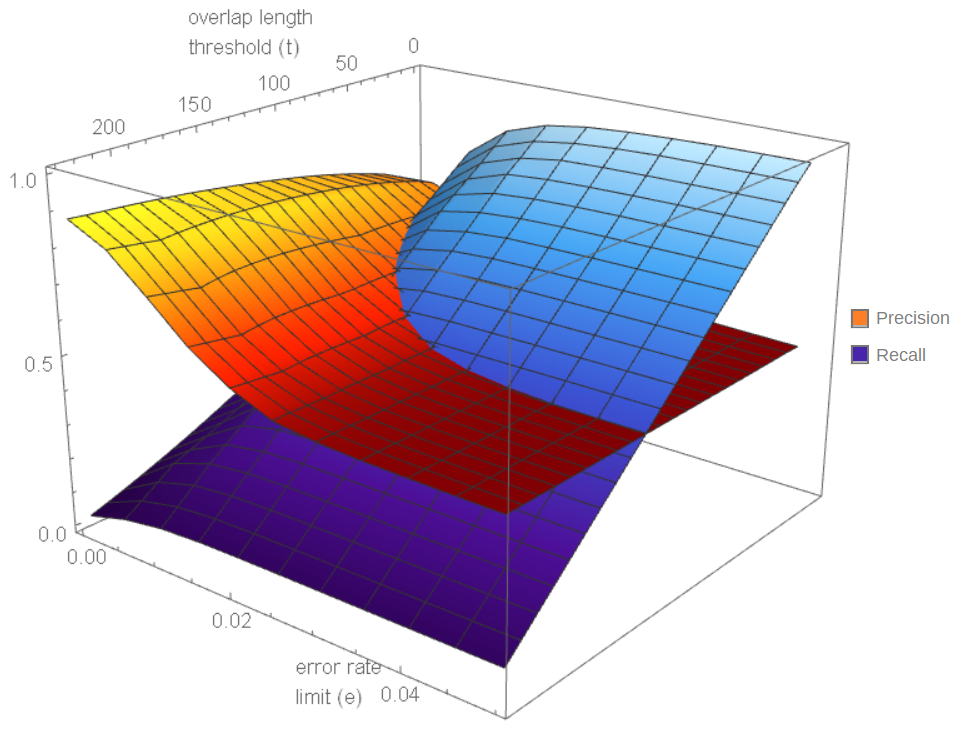
\includegraphics[width=1\linewidth]{images/phase1_A.png}
   \caption{}
\end{subfigure}

\begin{subfigure}[b]{0.8\textwidth}
   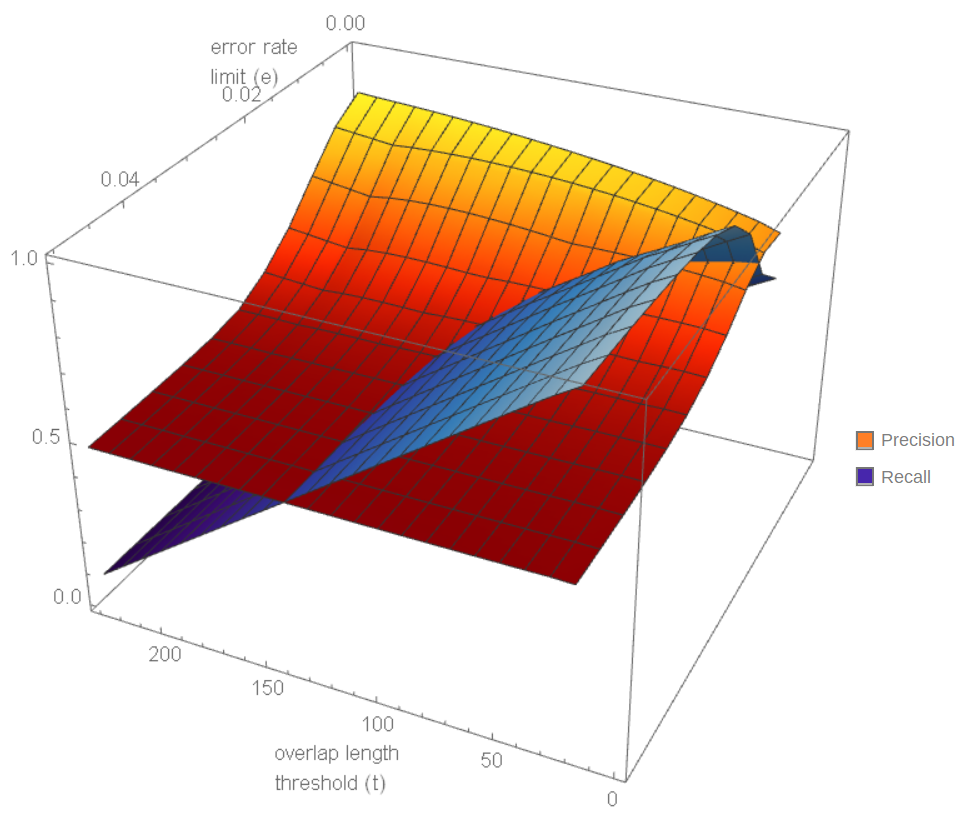
\includegraphics[width=1\linewidth]{images/phase1_B.png}
   \caption{}
\end{subfigure}

\caption[Precision and recall for output solution sets generated from runs using various \bfit{e} and \bfit{t} values.]{(a) Precision and recall for output solution sets generated from runs using various \bfit{e} and \bfit{t} values. (b) Alternative view.}
\label{fig:phase1_plots}
\end{figure}
\subsection{Observations}

As was expected, Figure \ref{fig:phase1_plots} shows that the solver achieves highest recall with restrictions relaxed as much as possible (low \bfit{t} and high \bfit{e}).

Outputs with the highest precision scores were the ones in which only \glspl{solution} \textit{highly} likely to be real were output.
\begin{enumerate}
\item Solutions that have longer overlaps are more likely to be real, explaining the correlation between high \bfit{t} and high precision.
\item Solutions that represent overlaps with very few errors are more likely to be real. Increased error blurs the distinction between different subsequences of the genome, increasing the number of false positives.
\end{enumerate}

Beyond approximately 3\% error, not much seems to change with respect to either metric, as can be seen in the `plateauing' of both recall and precision surfaces.

Clearly there is a trade-off between recall and precision to be considered when selecting one's input parameters. As very low values for either are highly undesirable, the values for run \textit{F-measures} in figure \ref{fig:phase1_02} give a view of the relative \textit{quality} of each run, factoring in the contributions of both recall and precision.


\begin{figure}[!htb]
\centering
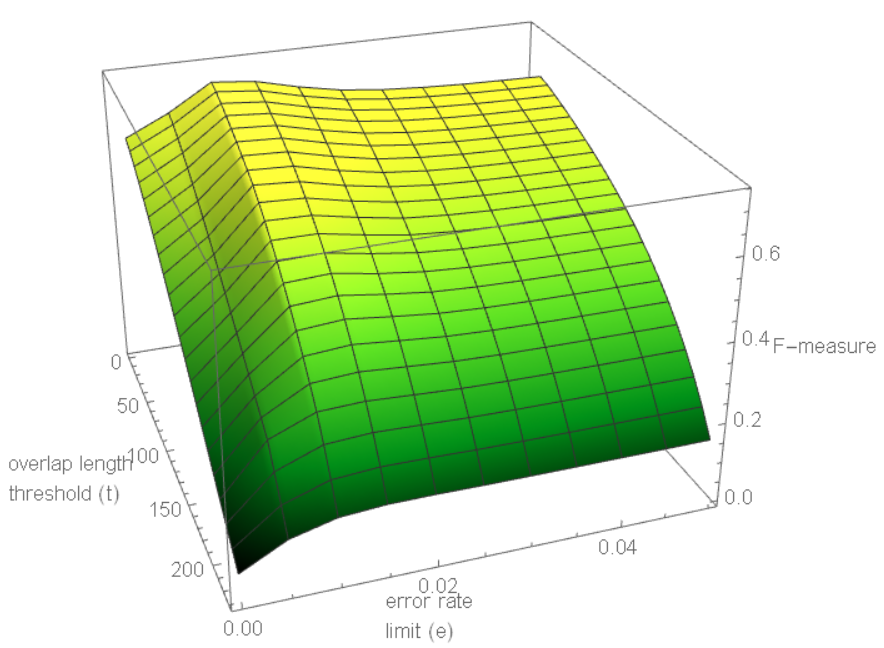
\includegraphics[width=0.9\textwidth]{images/fmeasure.png}
\caption{F-measure of output solution sets generated from runs using various \bfit{e} (error rate limit) and \bfit{t} (overlap threshold length) values.}
\label{fig:phase1_02}
\end{figure}

Use of shorter \bfit{t} appears to be consistently beneficial, and the choice of \bfit{e} seems optimal at approximately 1.2\% regardless of \bfit{t}. As exceptionally short overlap threshold of $< 80$ is undesirable for sequence assembly of viral genomes\footnote{See Section \ref{context} for more information on this choice of threshold.} (our primary use case), the optimal choice of parameters seems to be:
\begin{align*}
\bfit{t} &= 80\\
\bfit{e} &= 1.2\%
\end{align*}

\FloatBarrier

\section{Phase 2: Runtime Optimization Under Expected Conditions}
\label{phase2}

\subsection{Goal}
Experiments in this phase seek to tease out relationships between properties of the input data and runtime. Runtime on its own is a rather coarse measurement. For our \aspop{} solver, there are two logical means of fragmenting runtime into its principal components:

\begin{enumerate}
\item per \gls{suffix filter} block length

Patterns perform several \glspl{query} to the \gls{text index}, each with a different length of \gls{filter}. Aggregating like-sized filters will allow us a view into how filters of different lengths share the load of solving the problem, and identify algorithmic bottlenecks related to filters of only certain lengths.

\item per \gls{filter algorithm} step

The \gls{search step}'s runtime is a function of the shape of the query-search trees for each \gls{pattern}, which is in turn a function just about everything. The verification time is dependent on the number of \glspl{candidate} from the search step, as well as the rate at which candidates are \textit{spurious}.
\end{enumerate}

Very many properties can be extracted from a data set and reasoned over. Identifying the implications of properties that are \textit{intuitive} provides insight into what is actually happening inside the solver. Four such properties were identified and tested:

\begin{enumerate}
\item Genome Length

The length of the \gls{source genome} mostly affects the number of \glspl{read} in the data set without greatly\footnote{The impact of genome length on runtime is small when compared to a comparable increase in coverage, the most similar data set property. This is because both properties increase the number of reads to the same degree, but coverage usually introduces highly \textit{similar} reads leading to more text index hits and more overlap solutions.} impacting the number of overlaps per read. More reads also mean a longer \gls{text}, which has the side effect of more text index `hits', reducing pruning in query search trees. Unless otherwise specified, genome length is kept consistently at around 9600 nucleotides.

\item Read Length

Read length controls the \textit{maximum} length of a read (some fragments end up shorter). Read length is determined \textit{independently} to source genome length and \gls{coverage}; As the read length increases, the number of reads in the data set decreases. This is truly a measure of the \textit{fragmentation} of the source genome, not to be confused with coverage. Except in this experiment where it is the response variable, read length is consistently kept at approximately 250bp  (base pairs).

\item Coverage

Coverage is a measure of the number of \glspl{genome copy} composing the data set\footnote{Coverage has different specific definitions depending on the source. See the glossary definition of `coverage' for details. For our purpose, it is sufficient to consider coverage to be uniform across the length of the genome, being analogous to the count of genome copies in the data set.}. With a higher-coverage data set, there are more reads and more overlaps (in the \gls{search step} as well as the resulting \gls{solution} set). When not otherwise specified, experimental data sets have 500x coverage.

\item Divergence

If reads in a dataset are drawn from more than one source genome, one can reason about these genomes' divergence with respect to one another. Genomes with low divergence have a lot in common, and will contain more of the same substrings; A data set built from low-divergence genomes will likely result in more overlaps being found. For the coverage and divergence experiments, the data is drawn from real sources, with unknown constant values of coverage. For the other two experiments divergence is not defined, as only one source genome was used.

\end{enumerate}

\subsection{Experimental Design}
A battery of four experiment \textit{groups} tested the same target variables, but each time in response to a different \textit{data set property}. For each group, two experiments were performed:

\begin{enumerate}
\item Total runtimes (along with runtimes fragmented per \gls{filter algorithm} step) shown according to the given predictor variable.

\item Proportion of total runtime distributed across different \gls{filter} lengths, plotted across values of the predictor variable.
\end{enumerate}

% \FloatBarrier
\subsection{Results}
Figures \ref{fig:gnmlen} - \ref{fig:div} show the effect the various properties of the data set had on the runtime, as seen in two different partitions: per \gls{filter algorithm} step and per \gls{filter} blocks.



\begin{figure}
\centering
\makebox[\linewidth][c]{%
\begin{subfigure}[t]{.53\textwidth}
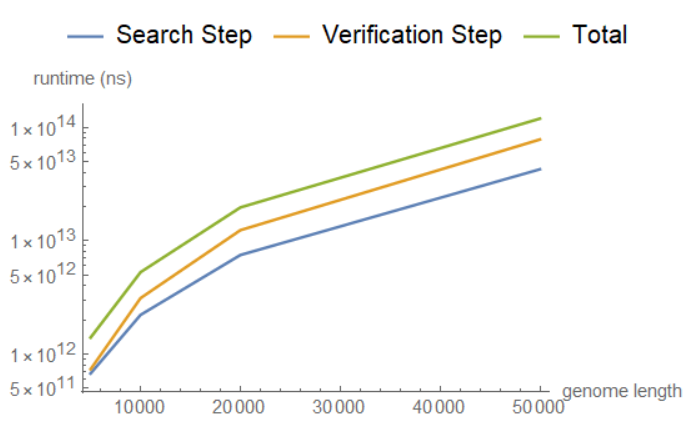
\includegraphics[width=1\linewidth]{images/gnmlen_a.png}
\caption{}
\end{subfigure}
~
\begin{subfigure}[t]{.53\textwidth}
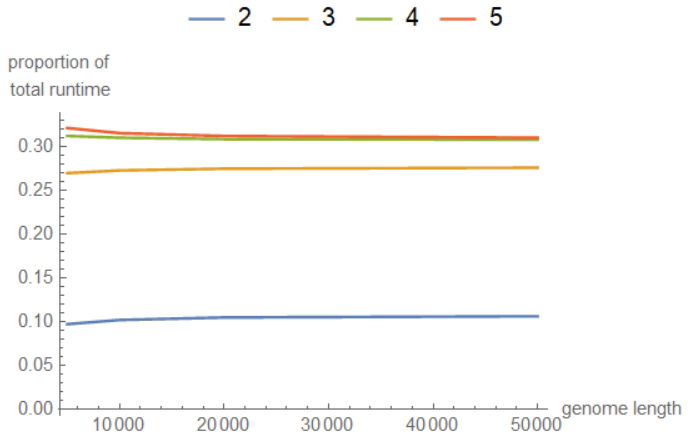
\includegraphics[width=1\linewidth]{images/gnmlen_b.png}
\caption{}
\end{subfigure}
}
\caption[Work time of \aspop{} solver runs partitioned into principal components, plotted as a function of \textit{genome length}]{Work of \aspop{} solver runs partitioned into principal components, plotted as a function of \textit{genome length}.\\(a) Total runtime (in nanoseconds) partitioned by filter algorithm step.\\(b) Runtime proportion partitioned by suffix filter block lengths.}
\label{fig:gnmlen}
\end{figure}



\begin{figure}
\centering
\makebox[\linewidth][c]{%
\begin{subfigure}[t]{.53\textwidth}
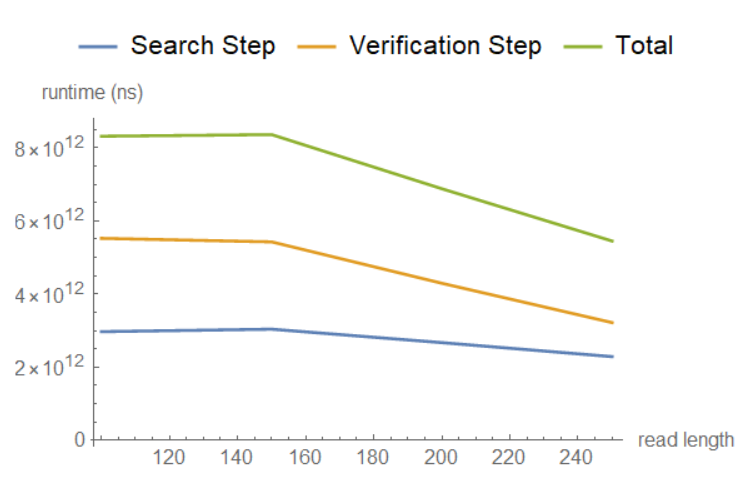
\includegraphics[width=1\linewidth]{images/rdlen_a.png}
\caption{}
\end{subfigure}
~
\begin{subfigure}[t]{.53\textwidth}
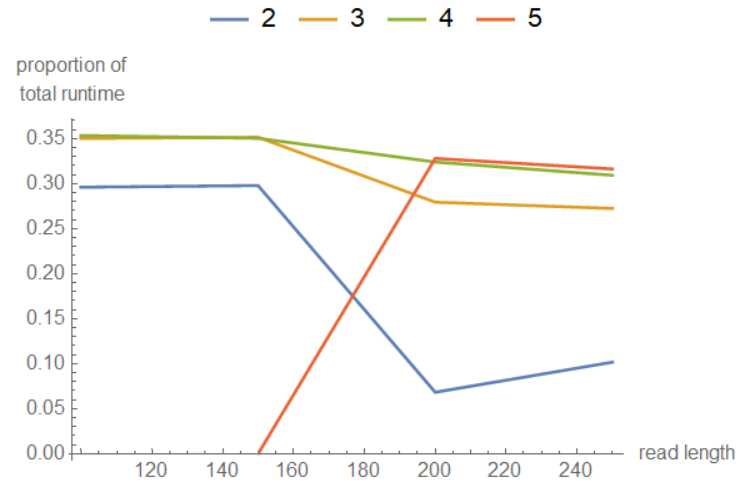
\includegraphics[width=1\linewidth]{images/rdlen_b.png}
\caption{}
\end{subfigure}
}
\caption[Work time of \aspop{} solver runs partitioned into principal components, plotted as a function of \textit{read length}]{Work of \aspop{} solver runs partitioned into principal components, plotted as a function of \textit{read length}.\\(a) Total runtime (in nanoseconds) partitioned by filter algorithm step.\\(b) Runtime proportion partitioned by suffix filter block lengths.}
\label{fig:rdlen}
\end{figure}



\begin{figure}
\centering
\makebox[\linewidth][c]{%
\begin{subfigure}[t]{.53\textwidth}
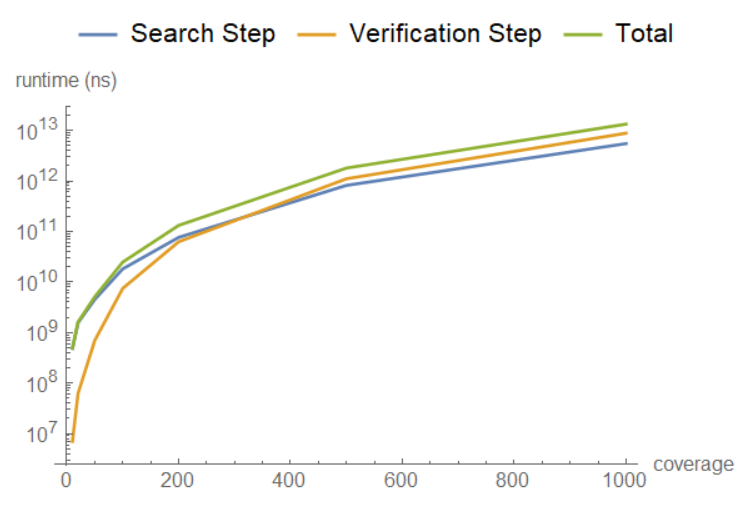
\includegraphics[width=1\linewidth]{images/cov_a.png}
\caption{}
\end{subfigure}
~
\begin{subfigure}[t]{.53\textwidth}
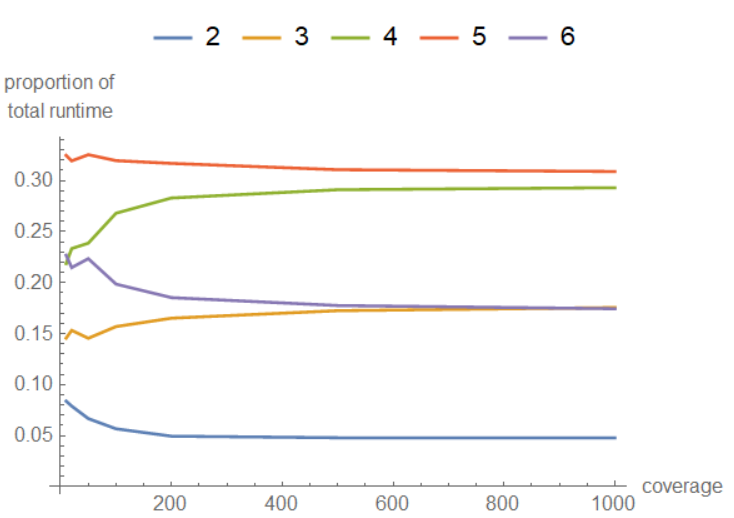
\includegraphics[width=1\linewidth]{images/cov_b.png}
\caption{}
\end{subfigure}
}
\caption[Work time of \aspop{} solver runs partitioned into principal components, plotted as a function of \textit{genome coverage}]{Work of \aspop{} solver runs partitioned into principal components, plotted as a function of \textit{genome coverage}.\\(a) Total runtime (in nanoseconds) partitioned by filter algorithm step.\\(b) Runtime proportion partitioned by suffix filter block lengths.}
\label{fig:cov}
\end{figure}



\begin{figure}
\centering
\makebox[\linewidth][c]{%
\begin{subfigure}[t]{.53\textwidth}
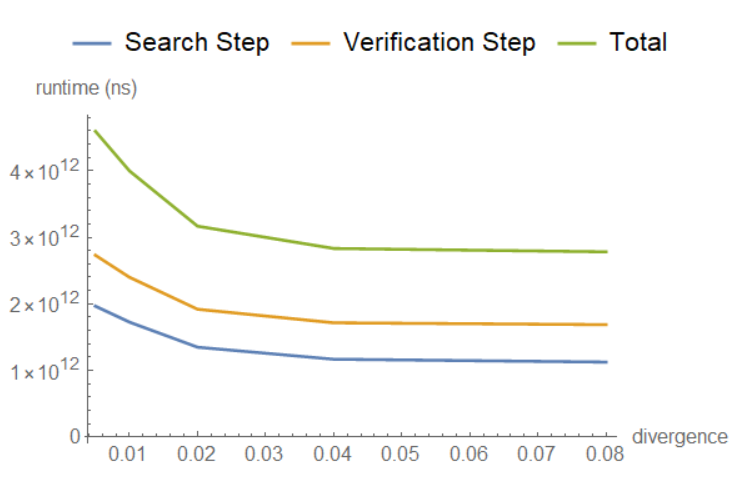
\includegraphics[width=1\linewidth]{images/div_a.png}
\caption{}
\end{subfigure}
~
\begin{subfigure}[t]{.53\textwidth}
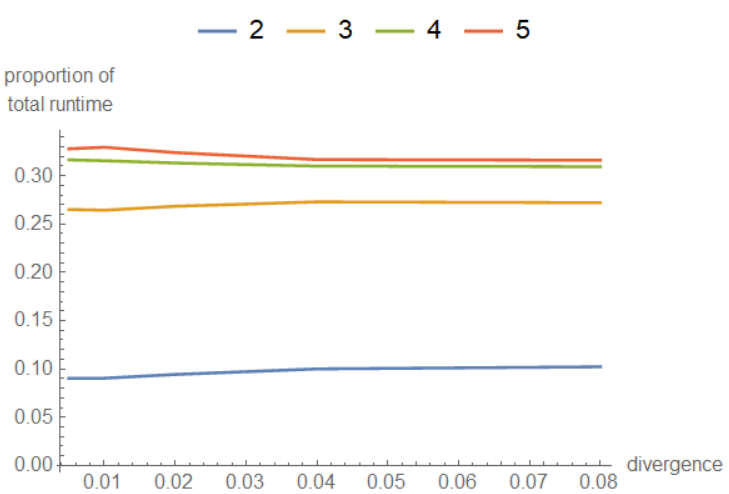
\includegraphics[width=1\linewidth]{images/div_b.png}
\caption{}
\end{subfigure}
}
\caption[Work time of \aspop{} solver runs partitioned into principal components, plotted as a function of \textit{genome divergence}]{Work of \aspop{} solver runs partitioned into principal components, plotted as a function of \textit{genome divergence}.\\(a) Total runtime (in nanoseconds) partitioned by filter algorithm step.\\(b) Runtime proportion partitioned by suffix filter block lengths.}
\label{fig:div}
\end{figure}

\FloatBarrier

\subsection{Observations}

Increased \textit{read length} in fig \ref{fig:rdlen} (a) demonstrated that for the same amount of data overall, the algorithm \textit{sped up} when faced with a smaller number of longer \glspl{read}, but not to an extreme extent. From (b), one can observe the longer \glspl{filter} beginning to `kick in' only for longer read lengths, as would be expected. It is notable here that filters took time roughly correspondent to their length. This is desirable behavior as it indicates that the workload is evenly distributed amongst filters (as much as their varying lengths will allow) and that no obvious niche cases are causing overwhelming slowdown. 
\begin{figure}[]
\centering
\makebox[\linewidth][c]{%
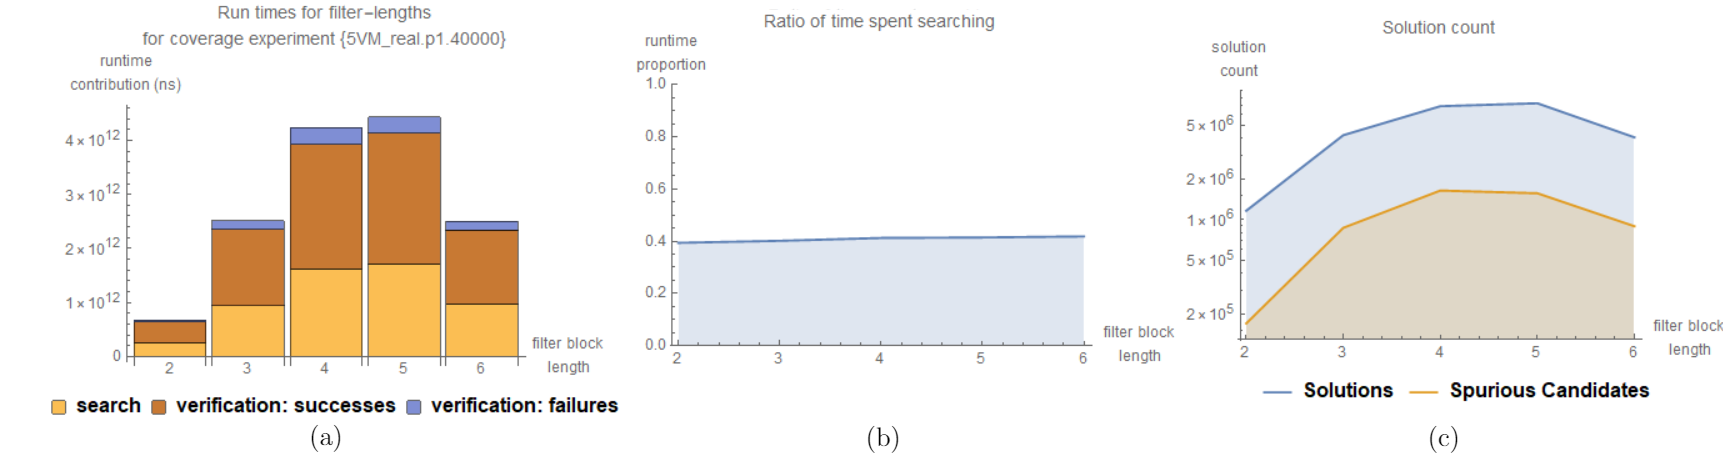
\includegraphics[width=1.3\textwidth]{images/cov40k_details.png}
}
\caption[Details of runtime for run `dataset\_coverage\_1000x'.]{Details of runtime for run `dataset\_coverage\_1000x'.\\(a) Runtime contributions for steps of the filter algorithm.\\(b) Ratio of time spent searching per filter block length.\\(c) Solution counts that did and did not verify per filter block length.}
\label{fig:cov40k_details}
\end{figure}
Increased \gls{coverage} proportionately increases the size of a data set, but increases the size of the \gls{solution} set super-linearly. As such, it is interesting to observe in Figure \ref{fig:cov} (a) that both steps of the \gls{filter algorithm} do not increase in lockstep, but the \gls{verification step} overtakes the \gls{search step} in runtime for high-coverage data. This was also visible in Figure \ref{fig:gnmlen} (a). Figure \ref{fig:cov} (b) Shows a trend for medium-length filters to contribute more to run time; Figure \ref{fig:cov40k_details} observes this in more detail, and shows that it is justified, with filters consistently spending more time working when they find more \glspl{solution}. Longest filters are shown to find fewer solutions than medium-length filters; This could be due to patterns differing in lengths and, consequently, several patterns simply not having a 6th filter to contribute to the overall runtime and solution set. The stabilizing proportions in Figure \ref{fig:cov} (b) are best explained as the law of large numbers at work; With low coverage (a smaller read set), the work contribution proportions are rather unstable. Why exactly these proportions seem to gravitate to fixed positions in a continuous direction and not in a zig-zagging fashion is unknown.




Increased \textit{divergence} in Figure \ref{fig:div} (a) was marked with a consistent reduction in overall runtime. This is to be expected as the data set's \glspl{source genome} have fewer overlaps in common, causing a more spindly search tree in the \gls{search step} as \glspl{match location} dry up. The  behavior of the individual filters remained relatively consistent for filters across the values of divergence. Figure \ref{fig:div} (b) shows that the distribution of work remains remarkably stable, maintaining the predicted relative positions across different solver executions.

\FloatBarrier
\section{Phase 3: Comparison to Other Solvers}
\label{phase3}

\subsection{Goal}
At the end of Phase 2 in Section \ref{phase2}, the implementation for our \aspop{} solver was considered final; This last phase tests how it compares to some existing solvers (namely \textsc{blast} and Minimap) in terms of \textit{output quality}\footnote{As with Phase 1 in Section \ref{phase1}, quality is defined in terms of \textit{F-measure} $=  2\cdot{}precision\cdot{}recall/(precision+recall)$.} and runtime in much the same way as in phase~1.

\textbf{Test 1} represents our primary focus on the use case of an \aspop{} solver in the context of viral genome assembly. Here, desirable \glspl{solution} only come from overlapping regions in the \glspl{source genome}; Only through the discovery of these `true' overlaps can the resulting assembly graph reconstruct these source genomes correctly. As such, the data set selected to represent this use case contains a mix of 5 viral strains. Overlaps found \textit{between} strains are not considered `true', instead counting as false positives and contributing to a diminished measure of precision.

\textbf{Test 2} compares the performance of our \aspop{} solver when applied to human DNA; The intention of this test is to check how runtime and output quality change when the solver is applied to a new type of data set with different properties.

\subsection{Experimental Design}

For each of the two tests, our \aspop{} solver, \textsc{blast} and Minimap were run on the data set sequentially. Many variations of this experiment are conceivable under these conditions, but for our purposes it was most interesting to test the performance of our system in conditions that were found in phase~1 to be conducive to finding the highest-quality solutions set for the purpose of viral genome assembly. As such, runs were done with error rate limit (\bfit{e}) $=$ 1.2\% and threshold overlap length (\bfit{t}) $=$ 80.

All solvers were run on a cluster computer of 24~Intel\textsuperscript{\textregistered} Xeon\textsuperscript{\textregistered} E52620-0s running at~2.00~GHz with 252~GB of storage. Each process was given 10~threads and sufficient free logical cores to run under negligible CPU contention.

The 5-mix of viral genomic data is taken from HXB2 (accession number K03455), available at the NCBI Reference database~\cite{ncbi}. It consists of a sample of 80,000 reads (approximately 2000x coverage) with most reads being of length 250bp.

The human DNA data is taken from Nisk.org's \textit{genome in a bottle} (Individual NA12878)~\cite{genomeinabottle}. Paired-end reads are 2x15 base-pairs at~30x coverage, but with \gls{read} ends truncated of extremely low confidence symbols (resulting in most reads being of length circa 150bp). These reads are taken from a 40,000bp-long subsequence of the MHC region, chromosome~6, base pairs 32,400,000~-~32,800,000.

\subsection{Results}\subsubsection{Viral Genome Data}
\label{p3_viral}

Figure \ref{fig:viral_timespace} shows the properties of the runs for all three solvers, such as the runtime\footnote{Note that runtime is measured \textit{cumulatively} for all running threads in all cores, while wall time is not. This means a well-parallelized program will have a long runtime, but short wall time.} (in terms of user time $+$ system time\footnote{`User time' refers to CPU time spent in user-mode code (outside the kernel) within the process. `System time' refers to CPU time spent in the kernel within the process.}), as well as the total elapsed `wall time' (real-world duration between start and finish of the execution). The peak space\footnote{Similar to runtime, memory usage can also be inflated with response to increased parallelism, as memory of all cores is counted together.} in memory used is also shown.

The Venn diagram given in Figure \ref{fig:viral_venn} shows the \textit{universe} of all unique overlap \glspl{solution} found between all three solvers; Solutions within the \textit{ground truth} set are also shown. Intuitively, a perfect solver's solution set would be equivalent to the ground truth set; Each excluded true solution decreases recall, and each included false solution decreases precision. 

Figure \ref{fig:prec_rec_f_p3} shows the values of recall, precision and \textit{f-measure} for all three solution sets with respect to the ground truth set.

\begin{figure}
\centering
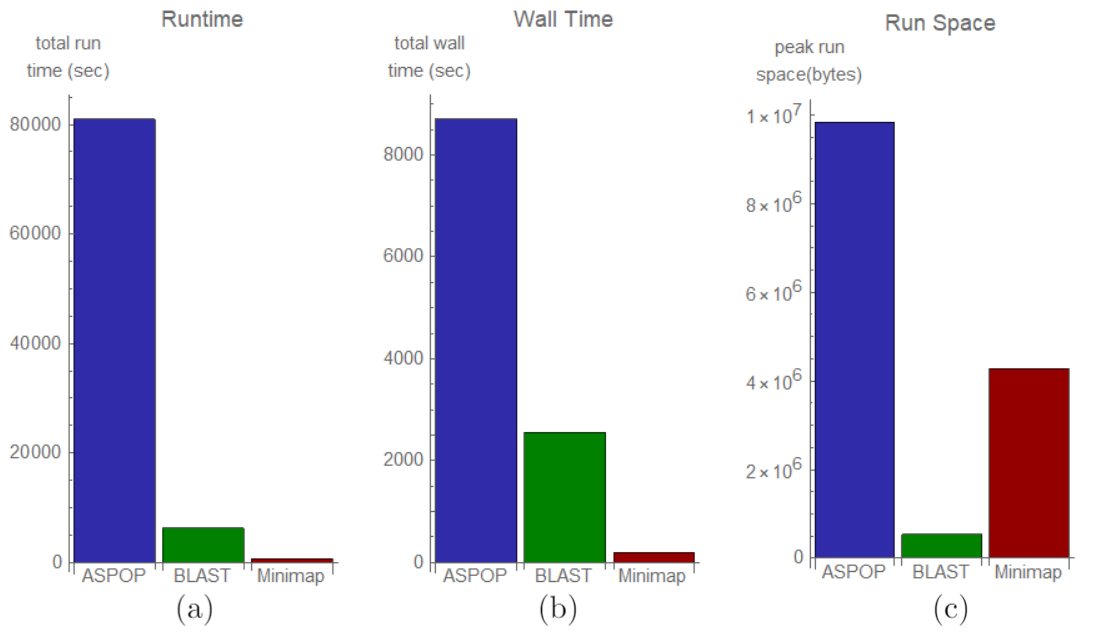
\includegraphics[width=0.85\linewidth]{images/time_space_v.png}
\caption[Time and space usages for runs of three \aspop{} solvers on a moderate data set containing a 5-strain mix of viral strains.]{Time and space usages for runs of three \aspop{} solvers on a moderate data set containing a 5-strain mix of viral strains.\\(a) Runtime of the solver in terms of system and user time in seconds\footnotemark{}.\\(b) Elapsed time as perceived externally in seconds.\\(c) Peak space required during solve in kb.}
\label{fig:viral_timespace}
\end{figure}

\FloatBarrier
\footnotetext{In the previous sections we have used nanosecond-granularity for time measurements, as they were made by a custom \aspop{} benchmarker able to measure time taken by components separately. For this test, we rely on linux's \url{/usr/bin/time} output, which uses second-granularity.}


\begin{figure}
\centering
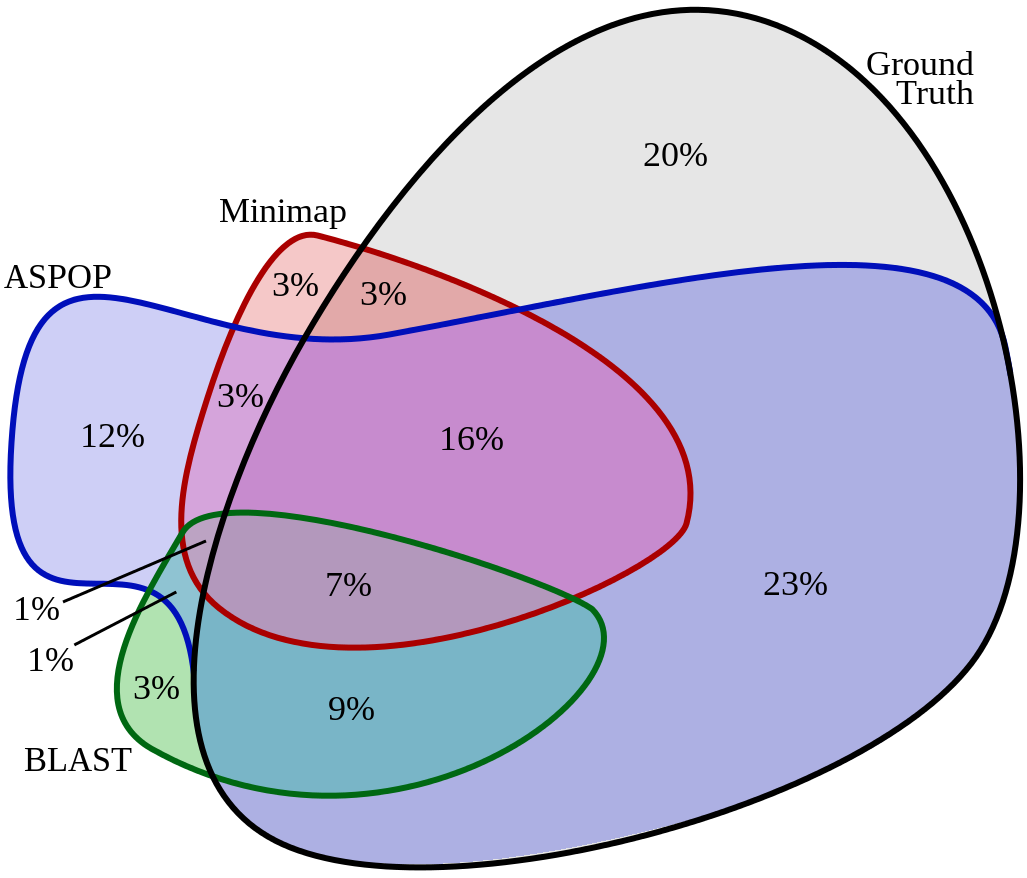
\includegraphics[width=0.55\linewidth]{images/viral_venn.png}
\caption[Venn diagram of solutions common between our \aspop{}, \textsc{blast} and Minimap against the \textit{ground truth} set for for a 5-strain viral mix data set]{Venn diagram of solutions found from a moderate 5-strain viral genome mix using our \aspop{} solver (blue), \textsc{blast} (green), Minimap (red) and the \textit{Ground Truth} (gray). Regions are labeled with the percentage of total solutions found, and are not necessarily to exact scale. Regions whose values round to $< 1\%$ of solutions are not labeled.}
\label{fig:viral_venn}
\end{figure}

\begin{figure}
\centering
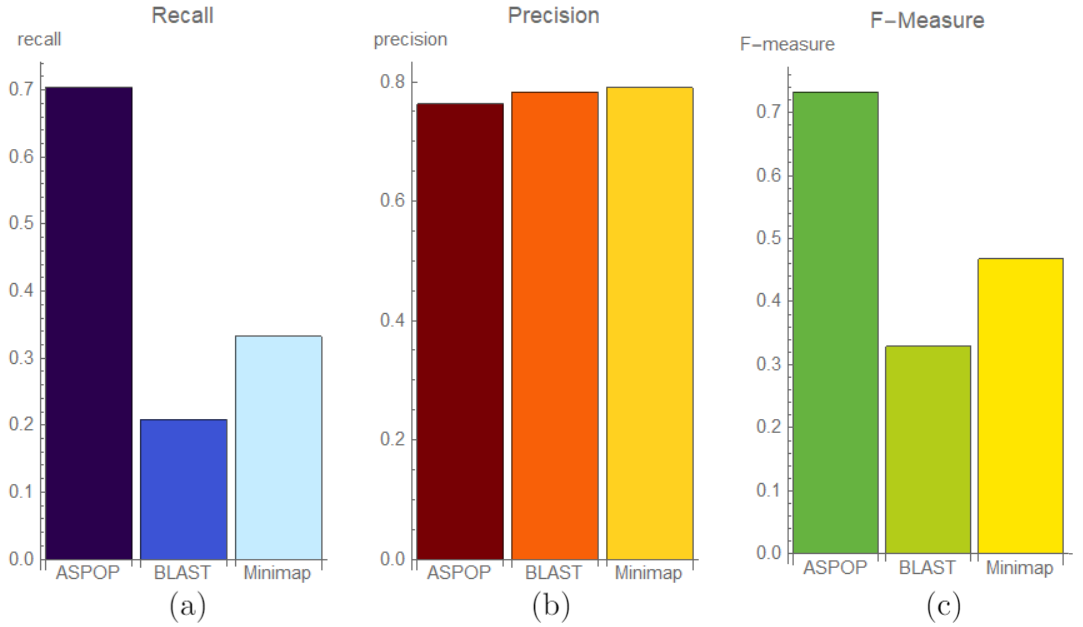
\includegraphics[width=0.9\linewidth]{images/prec_rec_f_p3.png}
\caption[Recall, precision, and f-measure for our \aspop{} solver, \textsc{blast} and Minimap running on a moderate 5-strain mix of viral data.]{Plots of (a) Recall (b) Precision and (c) F-measure for our \aspop{} solver, \textsc{blast} and Minimap running on a moderate 5-strain mix of viral data.}
\label{fig:prec_rec_f_p3}
\end{figure}


% \FloatBarrier


\subsubsection{Human Genome Data}
As in Section \ref{p3_viral} above, Figure \ref{fig:human_timespace} plots values\footnote{As in the previous section, the values of runtime and peak space are sensitive to parallelism. These solvers are parallelized to different degrees so it is important to interpret these measures in the context of wall time to gain a sense of the parallelism influencing the other values.} of runtime, wall time and peak space usage; In this experiment, the solvers were set on a data set containing \glspl{read} from human DNA.

Figure \ref{fig:human_venn} presents a Venn diagram of the \textit{universe} of \glspl{solution} found by all three solvers. Note that unlike the viral experiment, this data set has no known \textit{ground truth} set, as this is not simulated data under our control. As such, this diagram can only hint at the relationships between these solution sets, such as in which ways they are similar, different or how the size\footnote{\textsc{blast}, for instance, can output the same solution numerous times. Only \textit{unique} solutions are considered for these experiments.} between solution sets compare.



\begin{figure}
\centering
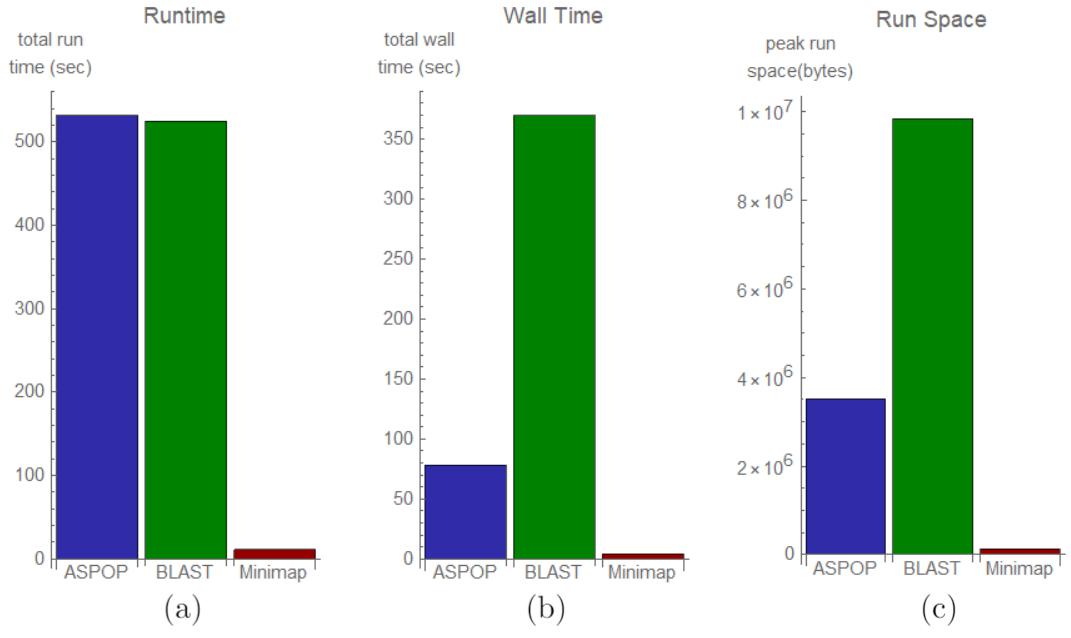
\includegraphics[width=0.9\linewidth]{images/time_space_h.png}
\caption[Time and space usages for runs of three \aspop{} solvers on a moderate data set containing a sample of human DNA]{Time and space usages for runs of three \aspop{} solvers on a moderate data set containing a sample of human DNA.\\(a) Runtime of the solver in terms of system and user time in seconds.\\(b) Elapsed time as perceived externally in seconds.\\(c) Peak space required during solve in kb.}
\label{fig:human_timespace}
\end{figure}

\begin{figure}
\centering
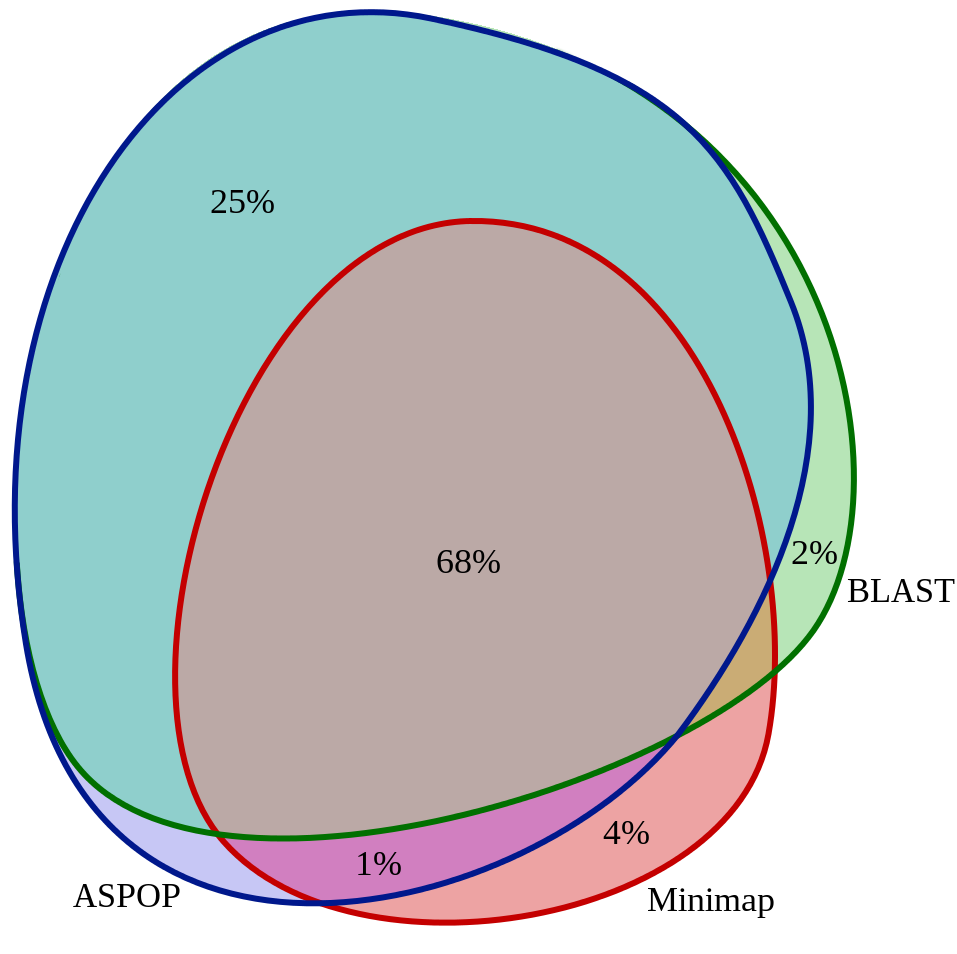
\includegraphics[width=0.5\linewidth]{images/human_venn.png}
\caption[Venn diagram of solutions common between our \aspop{}, \textsc{blast} and Minimap for for a data set of human DNA]{Venn diagram of solutions found from a small data set of human DNA using our \aspop{} solver (blue), \textsc{blast} (green) and Minimap (red). Regions are labeled with the percentage of total solutions found, and are not necessarily to exact scale. Regions whose values round to $< 1\%$ of solutions are not labeled.}
\label{fig:human_venn}
\end{figure}





\subsection{Observations}

Much can be ascertained about our \aspop{} solver, as well as its competitors, from the results of just these two experiments. It is immediately striking that Minimap is \textit{blazingly-fast} despite the fact that it didn't effectively make use of all 10 worker threads. Section \ref{fullmhc} shows that in a larger data set, Minimap's speed superiority becomes even more pronounced. In both cases, Minimap wrote \glspl{solution} in somewhere around 2\% of the time taken for our \aspop{} solver. However, overall, Minimap missed the largest percentage of solutions of all three solvers.

\textsc{blast} seemed to struggle with the human data, experiencing a spike in the wall time as well as peak run space. As this was not the case with the viral data, it seems likely that this is a result of blast struggling with the \textit{genome length}; This is a property with a large value for the human data set \textit{relative} to properties of the viral data set. \textsc{blast} consistently made the poorest use of parallelism, using an average of 230\% of CPU time even with 10 threads and an abundance of cores.

Our \aspop{} solver was generally the slowest solver of the three, specifically for the heftier viral data set. Our \aspop{} solver also had the largest space peak usage. However,  this is likely attributed to its thorough use of the available worker threads in tandem; With space requirements scaled to effective CPU usage, our solver had a smaller peak space usage than \textsc{blast} (and also Minimap in the human data experiment). On the other hand, our solver had the superior \textit{output quality}, represented by the F-measure for the viral experiment, where the \textit{ground truth} set was known. Although solvers were largely indistinguishable in terms of precision, the \aspop{} solver had the highest recall by far. This is almost certainly a direct result of the \gls{suffix filter} algorithm being \textit{exact}, instead of based on heuristics as with the other solvers.

For the \aspop{}, the choice of \bfit{e}$=1.2\%$ was optimal for the purpose of viral genome assembly. This might not necessarily be the case for the other solvers, lending credence to the notion that a user could achieve similar output quality to our solver using, for instance, Minimap but running it with more \textit{lenient} parameters (higher \bfit{e} or lower \bfit{t}); Minimap certainly has the time to spare for finding extra solutions. More work is needed to see if this holds. From what we know so far, it can however be presumed that running any solver with relaxed parameters results in decreased precision. For this reason, beating our solver's F-measure requires not only increased recall, but increased recall \textit{outweighing} the expected decreased precision.









\subsubsection{A Note about Runtime and Peak Run Space}
\label{note:runtime_runspace}

It is immediately apparent that the \aspop{} solver is the slowest; To make matters worse, for this experiment the \textsc{blast} solver had no choice but to find overlaps below the \textit{overlap length threshold} \bfit{t}, (As this is not an exposed parameter for \textsc{blast}) and to discard\footnote{In this decision there was a degree of compromise. If we kept the below-threshold overlaps we risked producing a \textsc{blast} solution set utterly incomparable to our \aspop{} solver's solution set. Alternatively, we could have removed the short solutions to better understand the sufficiently-long solutions that \textsc{blast} \textit{does} find. We concluded that the former option was the lesser of two evils.} them from the solution set. This was done as it is known from phase~1 of the experiments that short overlaps are undesirable even in ideal circumstances. The same can be said for the \textit{error rate limit} parameter \bfit{e} for Minimap, which is also not an exposed parameter for that solver; For both of the other solvers, this means that they are using time and space to find solutions that they are better off without (for the sake of this experiment at least). Unfortunately their natures are such that they cannot find their good solutions without finding these bad ones also. Thus, the runtimes and peak space measures for this phase's experiments should be taken with a grain of salt.

\FloatBarrier


\section{Auxiliary Experiments}
\label{phase_aux}

This section contains experiments and plots that were not sufficiently important, neither central to the focus of the thesis, or were otherwise \textit{auxiliary} to experiments in Sections \ref{phase1} - \ref{phase3}, but were still related and warranted being included.

\subsection{Partial Hamming Distance Measure}

From the experiments in phase~2, it became clear that for large data sets, which need speedup the most, a faster \gls{verification step} would make a considerable difference.

As discussed in Section \ref{unknown_b}, the \gls{search step} already performs some matching, and keeps track of \glspl{error}. After searching, \glspl{candidate} need to be verified to check if their overlaps' \textit{blind} components do not contain too many errors. A modification to the implementation was made to store information from the search step about the \textit{matched} component of the overlap (namely, its exact length and the counted errors within). With this knowledge, the verification step need only check the \gls{error distance} between blind components of overlaps, conceptually performing only a \textit{partial}~\gls{Hamming distance} calculation. Figure \ref{fig:partial_hamming} demonstrates the runtimes compared with and without this modification. As can be seen, the effects are consistently beneficial, but unfortunately negligible (runtime is only reduced by~2.27\% for 20,000x coverage). This is due to the fact that most of the time, the blind component is the majority of the overlap length anyway, and so the distance calculation remains largely the same. The extra space required to support this modification (2~extra numeric fields per \gls{candidate} structure) is not worth the meager speedup. As such, this modification was unfortunately rolled back.


\begin{figure}[!htb]
\centering
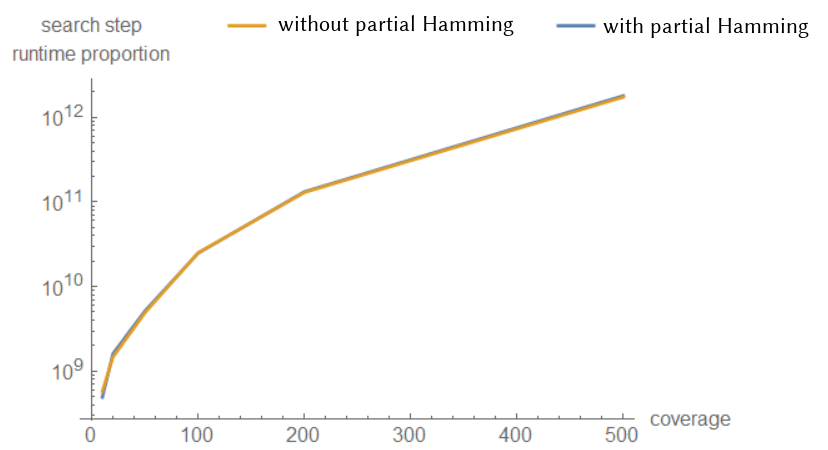
\includegraphics[width=.8\textwidth]{images/partial_hamming.png}
\caption{Comparative runtimes for executions with and without the `partial Hamming' modification across various values of coverage.}
\label{fig:partial_hamming}
\end{figure}

\subsection{Algorithm Extension Comparative Runtimes}
\label{extension_runtimes}

The \aspop{} implementation was built with the extensions from Section \ref{extensions} incorporated, enabled through the use of optional flags from the user. These extensions enrich the \gls{solution} set with new kinds of overlaps. The combination of several flags also yields unique solutions that cannot be found any other way. Of the three extensions (\gls{edit distance}, \glspl{reversal} and \glspl{inclusion}), use of reversals is most commonly advantageous for genome assembly. As such, it was used for tests throughout this work, but this need not be the case for the user.

Edit distance and inclusions are also not on by default; Although they are desirable in some cases, they are often not strictly necessary for sequence assembly, often avoided in part because they have a significant impact on runtime. Genome \gls{coverage} is shown to be a primary influence on runtime. As such, Figure \ref{fig:extensions} (a) shows the response of runtime to the use of the optional extensions, for otherwise the same problem instance; Although this figure seems to suggest that the enabling of edit distance simply scales up runtime by a constant factor, Figure \ref{fig:extensions} (b) shows that this is not the case. Using \textit{edit distance} fundamentally alters the ratios of work between the \gls{search step} and \gls{verification step} per run. Figure \ref{fig:cov} in Section \ref{phase2} would have us expect that (for edit distance disabled), the proportion of total runtime in Figure \ref{fig:extensions} (b) would fall below 50\% beyond the circa 500x \gls{coverage} mark. Unfortunately, with edit distance enabled, the runtime of this solver scales up considerably (as can be seen from (a)), forcing us to limit the coverage for this experiment to a maximum of 200x. We cannot extrapolate whether the edit-distance-enabled executions would experience runtimes with this same ratio of work in \gls{filter algorithm} steps as those of executions with edit distance disabled; Judging from the difference in behavior only within the 10x to 200x range, we would expect that the edit distance runs would likely not exhibit the `overtaking' behavior at 500x coverage seen in Figure \ref{fig:cov}.

\begin{figure}[!htb]
\centering
\makebox[\linewidth][c]{%
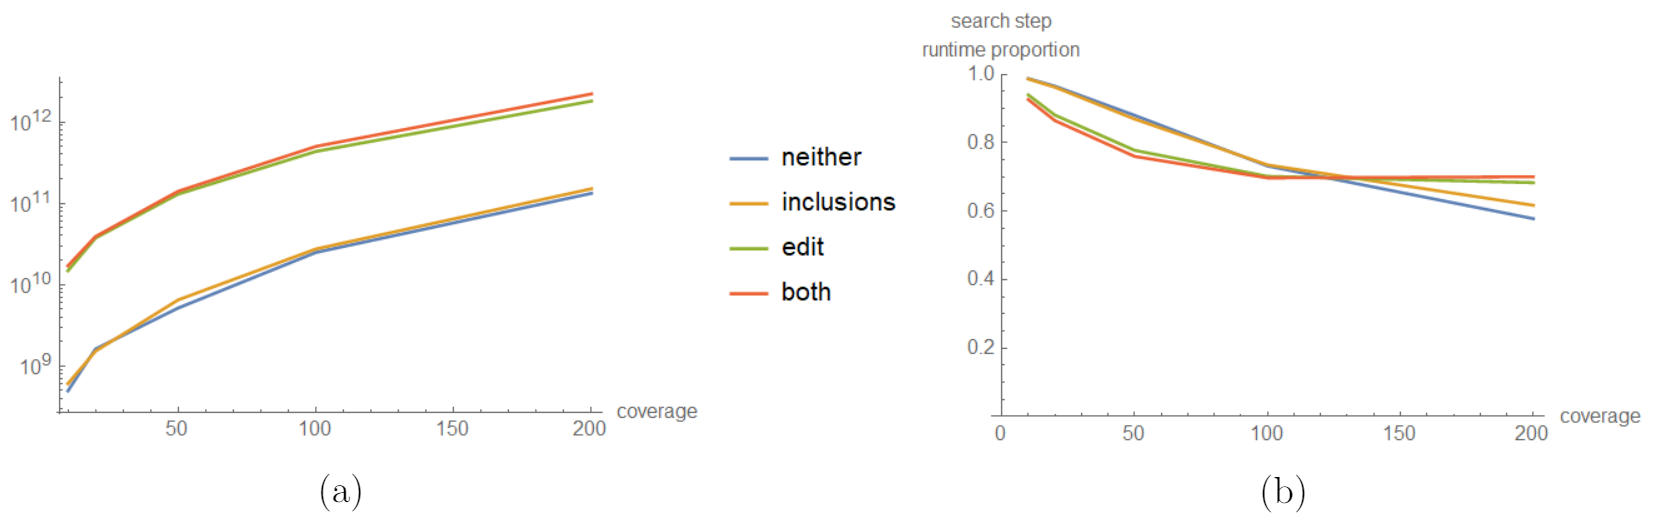
\includegraphics[width=1.15\textwidth]{images/extensions.png}
}
\caption[Runtime and runtime proportion of runs in response to coverage, with all combinations of optional flags enabling \textit{inclusions} and \textit{edit distance}.]{Runs in response to coverage, with all combinations of optional flags enabling \textit{inclusions} and \textit{edit distance} measured in terms of (a) Total runtime (b) Search step proportion of total runtime.}
\label{fig:extensions}
\end{figure}


\subsection{Runtime using \vali{}'s and Kucherov's Schemes}

Kucherov's \gls{suffix filter} algorithm introduced a new $S$ parameter (Explained in Section \ref{schemes:kuch}). In a nutshell, the choice of $S$ determines the number of \textit{redundant blocks} in the \gls{filter} associated with each search \gls{query} during the \gls{search step}. The trade-offs evident from choosing some $S$ over another yield an optimization problem, the nature of which is not immediately intuitive. 

Figure \ref{fig:schemes} demonstrates the runtime of executions using a modest viral-mix data set under the same parameters given by phase~1 in Section \ref{phase1}, in response to changing data set \gls{coverage}. \vali{}'s second algorithm resulted in significantly worse performance than Kucherov's with $S\leq{}2$ in all cases. This is consistent with Kucherov's own findings, as the \glspl{filter} in his scheme are more effective under these circumstances Additionally, Kucherov's algorithm makes use of a consistently-superior \gls{partitioning scheme}. The Kucherov run with $S=1$ behaves as the other Kucherov runs for extremely small data sets, but soon experiences \textit{extreme} slowdown in the higher-coverage run shown in Figure \ref{fig:schemes500}, much worse than that of the run using \vali{}'s second algorithm. This is a direct result of the \textit{short last block} problem explained in Section \ref{schemes:vali1} - \ref{schemes:kuch}. With $S=1$, no redundant blocks are given to the filters, resulting in the regrettable generation of hordes of \textit{spurious} \glspl{candidate}, as there are 0 completed blocks required by the \gls{candidate condition} in the \gls{query} search tree. This is especially evident in the shorter filters due to low $S$ values un-balancing the workload between filters. For this shorter run, \vali{}'s second algorithm still suffers  from its simple \gls{partitioning scheme}, relying on the work of more filters than would be necessary using Kucherov's partitioning scheme.

From all experiments conducted in this work, we observed a consistently superior runtime from Kucherov's algorithm with $S=2$. For this reason, $S=2$ is the value used elsewhere in the experiments. From Kucherov's own work, however, this trend might not continue to other problem instances with different properties beyond the bounds of our experiments \cite{kuch2014}.

\begin{figure}[!htb]
\centering
\makebox[\linewidth][c]{%
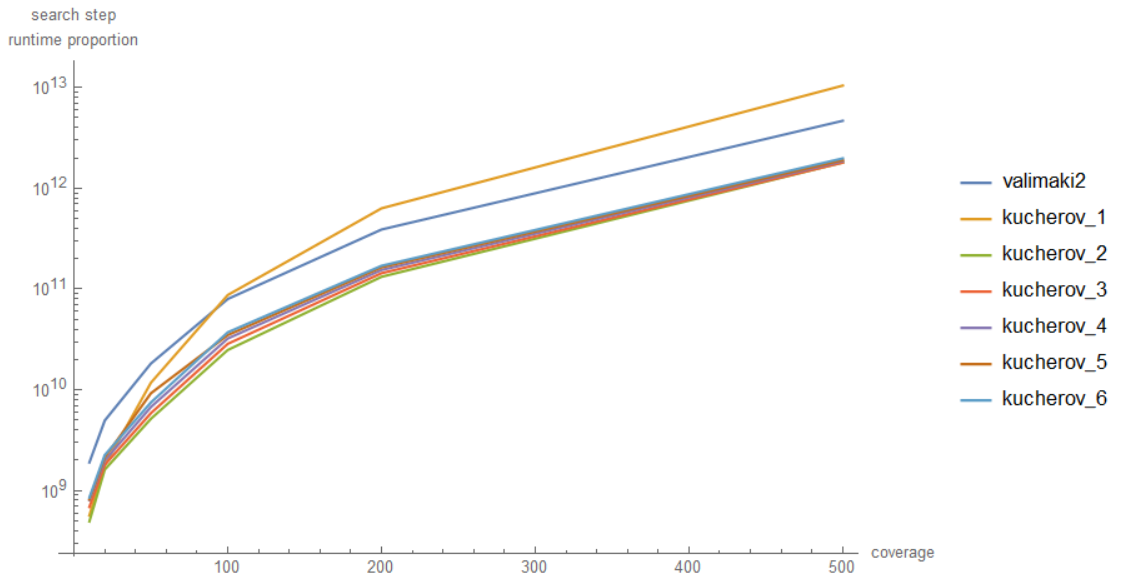
\includegraphics[width=1.0\textwidth]{images/schemes.png}
}
\caption{Comparative runtimes between \vali{}'s schemes, and Kucherov's schemes (using various values for parameter $S$), plotted in response to datasets with various values of coverage.}
\label{fig:schemes}
\end{figure}



\begin{figure}[!htb]
\centering
\makebox[\linewidth][c]{%
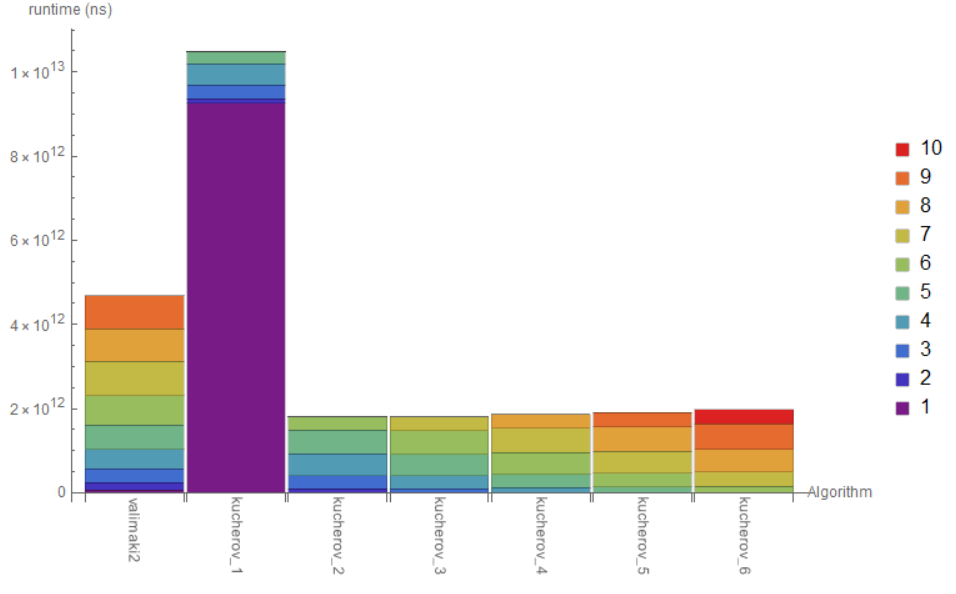
\includegraphics[width=0.9\textwidth]{images/schemes500.png}
}
\caption{Runtimes of filtering schemes of \vali{} and Kucherov, partitioned according to time per filter length, based on run `dataset\_coverage\_500x'.}
\label{fig:schemes500}
\end{figure}

\begin{figure}[!htb]
\centering
\makebox[\linewidth][c]{%
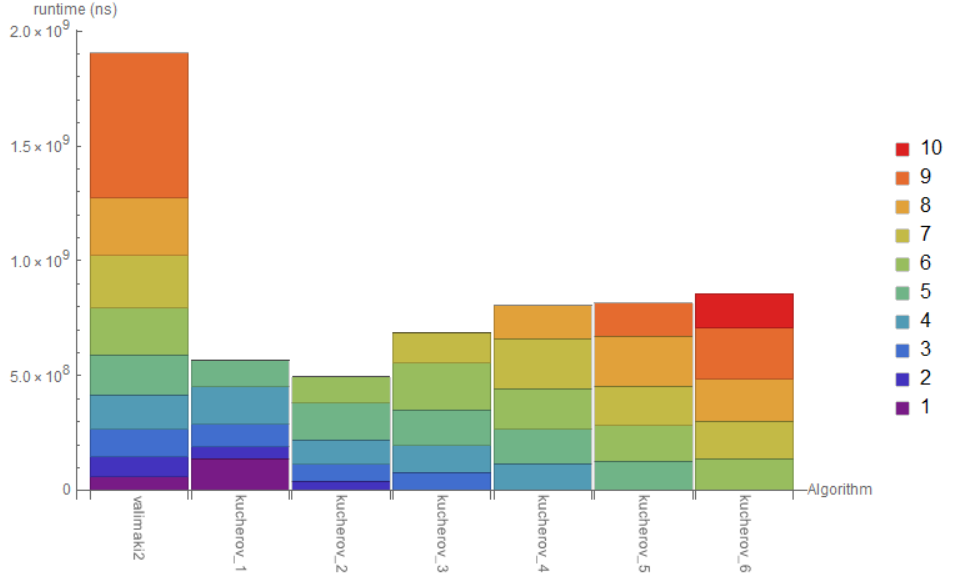
\includegraphics[width=0.9\textwidth]{images/schemes10.png}
}
\caption{Runtimes of filtering schemes of \vali{} and Kucherov, partitioned according to time per filter length, based on run `dataset\_coverage\_10x'.}
\label{fig:schemes10}
\end{figure}


\FloatBarrier
\subsection{Runtime on Full MHC Region of the Human Genome}
\label{fullmhc}

A final test of our program's speed tested its ability to handle larger data sets than were used for the numerous smaller tests. The the MHC region is located on chromosome 6, positions 28,477,797 - 33,448,354 (4,970,557 base pairs).

The run was under the same conditions as in phase 3 of the experiments, on a 24-core computer given 10 threads. After just under 25 hours, the program terminated with 1,051,648 solutions.

Unfortunately, the larger data sets showcased the differences in complexity classes between the solver. Compared to the second test in the phase 3 experiment, this data set came from a \gls{source genome} sequence 125x larger, and the run took 89,874 seconds up from 78. The run therefore took 1184x longer. By comparison, \textsc{blast} took 27 minutes to finish the same job, putting our \aspop{} solver to shame. Meanwhile, Minimap took just 34 seconds, now utterly blowing the competition out of the water in terms of speed.


\subsection{Prevalence of Pruned Nodes in Query Searches}
\label{aux:nodes}

This experiment intended to understand the practical difference between the worst-case and the typical case of the size of the \gls{query} search tree from the \gls{search step} of the \gls{suffix filter} algorithm. This section is somewhat meant as a \textit{foil} to the theoretical time complexity upper-bound defined in Section \ref{time_complexity}.

The implementation was temporarily modified to suppress pruning of \gls{query} search nodes that correspond with empty \gls{match location} sets. Instead, such nodes and all of their children are marked as `pruned' but otherwise retained. Counts of such nodes were printed to file, and the proportion computed for all searches in an execution in aggregate. It was immediately apparent during testing that the act of disabling pruning makes the solver significantly slower than before. Even the most trivial of data sets (40 \glspl{read} of 250bp) that usually takes less than a second to run didn't finish its execution in reasonable time. Thus, this experiment was run on a toy data set of generated reads with symbols sampled from a uniform distribution.

Table \ref{tab:nodes} shows the total prunable nodes in proportion to total nodes, using various combinations over ranges of \gls{read} length and number of input reads. No nodes are pruned for the 60-80 read length runs, as the search does not progress further than the first \gls{block} (with \bfit{t} set to 50). In runs with read length of 100 and beyond, an overwhelming proportion of the search tree is pruned. Naturally, the more massive search trees for longer read lengths produce more nodes; However, it becomes abundantly clear that as the search tree gets deeper, so too does the proportion of prunable nodes become even more overwhelming. In our experiment, the use of 5 significant figures was not sufficient to prevent this proportion from being indistinguishable from `1' for the largest read lengths. Although the number of reads indeed decreased the proportion of nodes pruned as expected (due to simply more \gls{text index} query hits), the proportion was modest, even between data sets with a 9-fold difference in number of reads.

As expected, the worst-case time complexity (which assumes only text index hits) is extremely pessimistic, and a user can expect a realistic execution to be \textit{lightening fast} by comparison.

\begin{table}
\centering
\caption[Proportion of nodes in query search trees pruned using Kucherov algorithm]{Proportion of nodes in query search trees pruned using Kucherov's algorithm on random data sets with $\bfit{e}=1.2\%$,  $S=2$, $\bfit{t}=50$ and reversals enabled. Read lengths (columns) ranged from 60 to 180; Number of input reads ranged from 10 to 90 (rows).\strut}
\begin{tabular}{|l||lllllll|}

\hline
 & 60 & 80 & 100 & 120 & 140 & 160 & 180 \\
\hline
\hline
10 & 0.0000 & 0.0000 & 0.9871 & 0.9909 & 0.9931 & 0.9945 & 1.0000 \\
30 & 0.0000 & 0.0000 & 0.9869 & 0.9908 & 0.9931 & 0.9945 & 1.0000 \\
90 & 0.0000 & 0.0000 & 0.9869 & 0.9908 & 0.9931 & 0.9945 & 1.0000 \\
\hline

\end{tabular}
\label{tab:nodes}
\end{table}
\chapter{Conclusion}

\vali{}'s 2012 publication revolutionized the exact \gls{suffix filter} algorithm for the \aspop{}~\cite{vali2012}. However, solving the `short last block' problem more elegantly, Kucherov's 2014 publication presented a new \gls{filtering scheme} and \gls{partitioning scheme} that facilitated massive speedup over and beyond that achieved by \vali{}~\cite{kuch2014}. Additionally, this new algorithm offered a means of calibration that promised to further increase speed when selected appropriately. However, without implementation, these newfound advances remained entirely theoretical.


Our new \aspop{} solver implementation was completed successfully, along with algorithm \textit{extensions} that support several new forms of output \glspl{solution}. These options are all exposed to the user, to be selected as desired. The open-source implementation was designed with future growth in mind, and is specifically structured to facilitate new \textit{schemes} that may arise from further development. Based on Kucherov's algorithm, the implementation in its current form is consistently observed to solve the same problem instances as the previous version of this solver in significantly less time; Most instances that once took a month to solve can be expected to finish in a day.

Unfortunately, when compared to existing heuristic \aspop{} solvers, \textsc{blast} and Minimap, our solver remains slow. This is especially true for data sets of extreme size, with \glspl{read} in excess of 80,000. As each solver has its own quirks, the specifics of the differences in runtimes between the solvers are highly variant in response to the properties of the input data. Although there are still many opportunities for optimization, this class of suffix filter algorithms already comes with a significant strength: \mbox{\textit{perfect~parallelism}}; This property is not ubiquitous amongst other algorithms for this problem. With many-core computers and large-scale distributed clusters becoming more economically feasible and abundant year by year, this property will only become more desirable, and could lead to an increased interest in developing solvers in this direction for this property alone.

\Glspl{filter algorithm} such as those in this work are conceptually complicated, leading to regrettable \textit{friction} when attempting to innovate. However, such complexity also provides many opportunities for future work, due to these algorithms still being young and poorly-understood. With the promise of improvements to come, along with the expected increase in value from their existing parallelizability, we see no reason that similar exact solvers shouldn't expect the current trend of accelerating speedup to continue.

A competitively-fast exact \aspop{} solver is a goal worth the pursuit. Such a solver guarantees an output set with reliable properties that can be explained in a sentence, free from all of the \textit{qualifying considerations} that are required for outputs of heuristic solvers. In addition, an exact solver is able to maximize recall without sacrificing precision. Regardless of the parameters for \gls{error rate} limit and overlap threshold length, heuristic solvers are never certain to find all of the `safest' overlap solutions (those most likely to correspond with real overlaps within a \gls{source genome}); Depending on the parameters used, heuristic solvers will find more `unsafe' solutions instead. This theory is consistent with the results of the 3rd phase of experiments (Section \ref{phase3}), which demonstrated that for the purpose of genome assembly, our solver reliably produced the highest-quality output set. For these reasons, further research should be done to push the speed of suffix filter algorithms to the next level, so that exact solvers can stand shoulder-to-shoulder with their established competitors as part of large-scale genome assemblers.
\chapter{Future Work}
With such a complex system and such large data sets, very many experiments can be concocted that would each be more interesting than the last. Additionally, there is a lot of potential for improvement of our solver through improvement of the implementation itself. Unfortunately, due to a shortage of time, exploration of all of these avenues was not possible. As such, this section highlights a number of potential focal points that seem likely to result in fruitful future works.

\section{Future Implementation}

Initially, it was intended for a greater proportion of time to be spent experimenting with the effects of using different (and perhaps novel) \glspl{partitioning scheme}. Even comparison against provably-worse schemes than that of Kucherov's algorithm would give a lot of information about the nature of the relationship between the \gls{pattern} partition and runtime.


Our \aspop{} solver implementation is not capable of efficiently dealing with \glspl{indel} at the moment, and there is unlikely to be a cheap `silver bullet' solution that will change that any time soon. In this facet, competitors such as \textsc{blast} are likely to keep their advantage for the time being. At least in the face of short-\gls{read} sequence data, so far the use of indels does not appear to help find more `real' overlaps from the same source genome very often, and in fact consideration of indels can do more harm than good \textit{aside} from the increased runtime. Read data usually contains indels so rarely (circa 10 times rarer than \glspl{substitution} \cite{err_rates}), that the bulk of indel-containing \glspl{solution} mostly just inflate \textit{false positive} rates, causing detriment to later steps of the assembly process. This realization came late in the progress of this project, with a great deal of time already having been spent trying to make indel mode efficient (to little avail). At least in its current state, indel mode is functional in the event of small data sets or many cores.


More drastic changes in approach might be necessary to dramatically increase the speed of Kucherov's algorithm further. However, due to its complicated nature, there are a number of interesting projects that could be borne of this one. For example, in-depth knowledge of systems programming would allow someone with the right skill-set to squeeze more speedup out of the same algorithm. Another viable approach might be a more \textit{specialized} implementation, stripping away the modularity required to support optional running modes and the swappable \textit{mode} component described in Section~\ref{structure}. A leaner, purpose-built implementation might not only be faster on paper, but would also be able to skip some minor internal trans-representation conversion steps, exposing some opportunities for clever tricks that would push efficiency to the next level.

Development of a viable auxiliary \textit{correctness-checker} was considered for this project, but it was ultimately scrapped due to time constraints. This program would have allowed automated testing of the correctness of the \gls{suffix filter} algorithm's \textit{mode} module. This would allow the user to tinker with the code for \glspl{filter} and \gls{pattern} partitioning, with the  correctness-checker ensuring that the algorithm remains exact. This would allow for the kind of rapid iteration that might lead to a new breakthrough for the \gls{filter algorithm}, much in the way \kark{} created suffix filters from the existing \glspl{substring filter}. 

\section{Future Experimentation}

There was not enough time to test the effects of using optional \glspl{inclusion} on the output quality, much as it was done in Section~\ref{phase1}. It would also be interesting to understand their usefulness for the sequence assembly process. Information about these ramifications would help to clarify in which cases the user should enable inclusions. The same could be said with respect to \glspl{reversal}; Although the resulting doubling of the number of searched \glspl{read} is clear, it is not apparent to which extent these reversed reads reduce the pruning of nodes in \gls{query} search trees, as was tested \textit{without} considering reversals in Section~\ref{aux:nodes}.

It would be interesting to explore the behavior of all three solvers in the face of large data sets of different \textit{kinds} of data to identify the niches in which each solver shines.

In the spirit of the experiments of phase~1 (Section~\ref{phase2}), a more exhaustive exploration of which parameters to select for different applications would also be quite illuminating; This could help to specialize the advisable parameter settings for different possible use cases.



%now enable appendix numbering format and include any appendices
% \appendix
% \include{appendix1}
% \include{appendix2}

\appendix
\chapter{Appendix}
 \label{appendix}
\section{Auxiliary Information}
 \label{aux_info}

\subsection{Text Indices \& FM-Index}
\label{fmindex}

\Glspl{text index} (also called \textit{substring indices} or \textit{full-text indices}) are data structures specifically meant for finding substrings within a \gls{text} in sub-linear time. They are explained in detail in a referenced survey paper~\cite{fmfordummies}. As the initialization of the text is costly, text indices are only worthwhile when numerous \glspl{query} for substrings of the same text are expected. Text indices work by traversing the contents of the given text and making annotations or restructuring them as necessary to `front-load' the work that queries would need to do; This can be thought of as `constructing a text index around a text'.
 
The FM-Index primarily uses a Burrows-Wheeler-Transformed text string as well as as \textit{suffix index} to store the relevant information. The details of Burrows-Wheeler Transform are briefly summarized in \ref{bwt}. Intuitively, the transformed text encodes which symbols \textit{precede} one another within the original text string. Due to its structure, all \glspl{match location} for a query are always `represented' by adjacent symbols in this \textsc{bwt}-string, allowing the full set of match locations to be stored in just two numbers: the bounds of a range. The index incrementally matches to a \gls{query} from back to front by essentially \textit{specifying} the matched substring, updating the match set range accordingly; At each step, the range represents the occurrences of the suffix of the query already matched. Each step of the matching process calls a subroutine often called `rank' or `occurrences', necessary for finding the range of the next node in the index search tree. The cost of this rank call varies depending on source; Often it is given as a \textit{large constant}.
 
The nature of the \textsc{bwt} facilitates \textit{backwards search}, specifying the query string from back to front. Many relevant procedures involving this search conceptually reason using a \textit{forwards search}, which differs only in the order of traversal. The iterative steps of this search are integrally-related to the partition \glspl{block} and \glspl{filter} used in the \aspop{} solution; These notions are usually described \textit{forwards} in the literature. A forwards search in the FM-Index can be simulated by initializing the text index on a \textit{reversed} text; These counter-intuitive representations are encapsulated inside the FM-Index and are not visible outside of it. For more details about how the implementation deals with this detail, see Section \ref{own_impl_search_dir}.


\subsection{Burrows-Wheeler Transform}
\label{bwt}

\textit{Burrows-Wheeler Transform} (or \textsc{bwt} for short) is a procedure that returns a permutation of some input string $s$ with specific desirable properties. The transformation can also be reverted if necessary. \textsc{bwt} strings tend to contain many \textit{runs} of the same symbols, allowing for some compression potential. Additionally, and more importantly for our purposes, the transformed string $s'$ is able to encode additional information about the sequence of characters in the original string without taking up any extra space.
 
For the procedure, $s$ is assumed to be end-delimited by an extra-alphabetic symbol, conventionally `\$'. The \textsc{bwt}-string is computed as follows:

\begin{enumerate}
\item For all rotations of $s$, create a row in a matrix, where a \textit{rotation} is $s[i+1,|s|]s[1,i]$ for $1\leq{} i \leq{|s|}$.
\item Sort the rows of the matrix according to a left-to-right lexicographic ordering of their symbols.
\item Return $s'$, the string represented by the symbols in the last column of the matrix, read from top to bottom.
\end{enumerate}

Ultimately, only $s'$ is retained, with the rest of the matrix and other intermediate data discarded. As $s$ and $s'$ are composed of columns from this same matrix, clearly $|s|=|s'|$.

If necessary, the first column of the matrix can be reacquired by simply sorting the symbols in $s'$. Then $s$ can be reconstructed from back to front beginning with the terminal `\$', with all preceding symbols `looked up' using the first and last columns of the \textsc{bw}-matrix.



% \section{Experiment Raw Data}

% \subsection{Phase 1}

% \begin{sidewaystable}[!htbp]
%     \centering
%     \caption{Phase 1 false negative counts of \aspop{} solver runs across multiple values of \bfit{t} and \bfit{e}. True solution set contains 4854458 elements.}
%     \label{table:phase1neg}
% \csvautobooktabular{data/negs_trans_labels.csv}
% \end{sidewaystable}

% \begin{sidewaystable}[!htbp]
%     \centering
%     \caption{Phase 1 false positive counts of \aspop{} solver runs across multiple values of \bfit{t} and \bfit{e}.}
%     \label{table:phase1pos}
% \csvautobooktabular{data/poss_trans_labels.csv}
% \end{sidewaystable}

\newpage
\section{Thesis Task Breakdown}

\begin{figure}[!htb]
\centering
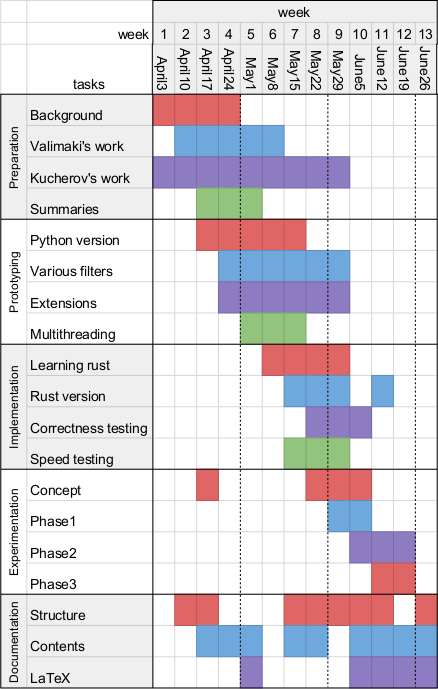
\includegraphics[width=0.7\textwidth]{images/sheet.png}
\caption{Thesis task breakdown per week.}
\label{fig:planner}
\end{figure}


\printglossaries

%next line adds the Bibliography to the contents page
\addcontentsline{toc}{chapter}{Bibliography}
%uncomment next line to change bibliography name to references
%\renewcommand{\bibname}{References}
\bibliography{refs}        %use a bibtex bibliography file refs.bib
\bibliographystyle{plain}  %use the plain bibliography style

\end{document}
